%2multibyte Version: 5.50.0.2960 CodePage: 936

\documentclass[notes=show]{beamer}
%%%%%%%%%%%%%%%%%%%%%%%%%%%%%%%%%%%%%%%%%%%%%%%%%%%%%%%%%%%%%%%%%%%%%%%%%%%%%%%%%%%%%%%%%%%%%%%%%%%%%%%%%%%%%%%%%%%%%%%%%%%%%%%%%%%%%%%%%%%%%%%%%%%%%%%%%%%%%%%%%%%%%%%%%%%%%%%%%%%%%%%%%%%%%%%%%%%%%%%%%%%%%%%%%%%%%%%%%%%%%%%%%%%%%%%%%%%%%%%%%%%%%%%%%%%%
\usepackage{amssymb}
\usepackage{graphicx}
\usepackage{mathpazo}
\usepackage{hyperref}
\usepackage{multimedia}

%TCIDATA{OutputFilter=LATEX.DLL}
%TCIDATA{Version=5.50.0.2960}
%TCIDATA{Codepage=936}
%TCIDATA{<META NAME="SaveForMode" CONTENT="2">}
%TCIDATA{BibliographyScheme=Manual}
%TCIDATA{Created=Monday, January 02, 2012 10:10:09}
%TCIDATA{LastRevised=Wednesday, November 06, 2013 07:37:45}
%TCIDATA{<META NAME="GraphicsSave" CONTENT="32">}
%TCIDATA{<META NAME="DocumentShell" CONTENT="Other Documents\SW\Slides - Beamer">}
%TCIDATA{CSTFile=beamer.cst}

\newenvironment{stepenumerate}{\begin{enumerate}[<+->]}{\end{enumerate}}
\newenvironment{stepitemize}{\begin{itemize}[<+->]}{\end{itemize} }
\newenvironment{stepenumeratewithalert}{\begin{enumerate}[<+-| alert@+>]}{\end{enumerate}}
\newenvironment{stepitemizewithalert}{\begin{itemize}[<+-| alert@+>]}{\end{itemize} }
\usetheme{Madrid}
% Macros for Scientific Word and Scientific WorkPlace 5.5 documents saved with the LaTeX filter.
% Copyright (C) 2005 Mackichan Software, Inc.

\typeout{TCILATEX Macros for Scientific Word and Scientific WorkPlace 5.5 <06 Oct 2005>.}
\typeout{NOTICE:  This macro file is NOT proprietary and may be 
freely copied and distributed.}
%
\makeatletter

%%%%%%%%%%%%%%%%%%%%%
% pdfTeX related.
\ifx\pdfoutput\relax\let\pdfoutput=\undefined\fi
\newcount\msipdfoutput
\ifx\pdfoutput\undefined
\else
 \ifcase\pdfoutput
 \else 
    \msipdfoutput=1
    \ifx\paperwidth\undefined
    \else
      \ifdim\paperheight=0pt\relax
      \else
        \pdfpageheight\paperheight
      \fi
      \ifdim\paperwidth=0pt\relax
      \else
        \pdfpagewidth\paperwidth
      \fi
    \fi
  \fi  
\fi

%%%%%%%%%%%%%%%%%%%%%
% FMTeXButton
% This is used for putting TeXButtons in the 
% frontmatter of a document. Add a line like
% \QTagDef{FMTeXButton}{101}{} to the filter 
% section of the cst being used. Also add a
% new section containing:
%     [f_101]
%     ALIAS=FMTexButton
%     TAG_TYPE=FIELD
%     TAG_LEADIN=TeX Button:
%
% It also works to put \defs in the preamble after 
% the \input tcilatex
\def\FMTeXButton#1{#1}
%
%%%%%%%%%%%%%%%%%%%%%%
% macros for time
\newcount\@hour\newcount\@minute\chardef\@x10\chardef\@xv60
\def\tcitime{
\def\@time{%
  \@minute\time\@hour\@minute\divide\@hour\@xv
  \ifnum\@hour<\@x 0\fi\the\@hour:%
  \multiply\@hour\@xv\advance\@minute-\@hour
  \ifnum\@minute<\@x 0\fi\the\@minute
  }}%

%%%%%%%%%%%%%%%%%%%%%%
% macro for hyperref and msihyperref
%\@ifundefined{hyperref}{\def\hyperref#1#2#3#4{#2\ref{#4}#3}}{}

\def\x@hyperref#1#2#3{%
   % Turn off various catcodes before reading parameter 4
   \catcode`\~ = 12
   \catcode`\$ = 12
   \catcode`\_ = 12
   \catcode`\# = 12
   \catcode`\& = 12
   \catcode`\% = 12
   \y@hyperref{#1}{#2}{#3}%
}

\def\y@hyperref#1#2#3#4{%
   #2\ref{#4}#3
   \catcode`\~ = 13
   \catcode`\$ = 3
   \catcode`\_ = 8
   \catcode`\# = 6
   \catcode`\& = 4
   \catcode`\% = 14
}

\@ifundefined{hyperref}{\let\hyperref\x@hyperref}{}
\@ifundefined{msihyperref}{\let\msihyperref\x@hyperref}{}




% macro for external program call
\@ifundefined{qExtProgCall}{\def\qExtProgCall#1#2#3#4#5#6{\relax}}{}
%%%%%%%%%%%%%%%%%%%%%%
%
% macros for graphics
%
\def\FILENAME#1{#1}%
%
\def\QCTOpt[#1]#2{%
  \def\QCTOptB{#1}
  \def\QCTOptA{#2}
}
\def\QCTNOpt#1{%
  \def\QCTOptA{#1}
  \let\QCTOptB\empty
}
\def\Qct{%
  \@ifnextchar[{%
    \QCTOpt}{\QCTNOpt}
}
\def\QCBOpt[#1]#2{%
  \def\QCBOptB{#1}%
  \def\QCBOptA{#2}%
}
\def\QCBNOpt#1{%
  \def\QCBOptA{#1}%
  \let\QCBOptB\empty
}
\def\Qcb{%
  \@ifnextchar[{%
    \QCBOpt}{\QCBNOpt}%
}
\def\PrepCapArgs{%
  \ifx\QCBOptA\empty
    \ifx\QCTOptA\empty
      {}%
    \else
      \ifx\QCTOptB\empty
        {\QCTOptA}%
      \else
        [\QCTOptB]{\QCTOptA}%
      \fi
    \fi
  \else
    \ifx\QCBOptA\empty
      {}%
    \else
      \ifx\QCBOptB\empty
        {\QCBOptA}%
      \else
        [\QCBOptB]{\QCBOptA}%
      \fi
    \fi
  \fi
}
\newcount\GRAPHICSTYPE
%\GRAPHICSTYPE 0 is for TurboTeX
%\GRAPHICSTYPE 1 is for DVIWindo (PostScript)
%%%(removed)%\GRAPHICSTYPE 2 is for psfig (PostScript)
\GRAPHICSTYPE=\z@
\def\GRAPHICSPS#1{%
 \ifcase\GRAPHICSTYPE%\GRAPHICSTYPE=0
   \special{ps: #1}%
 \or%\GRAPHICSTYPE=1
   \special{language "PS", include "#1"}%
%%%\or%\GRAPHICSTYPE=2
%%%  #1%
 \fi
}%
%
\def\GRAPHICSHP#1{\special{include #1}}%
%
% \graffile{ body }                                  %#1
%          { contentswidth (scalar)  }               %#2
%          { contentsheight (scalar) }               %#3
%          { vertical shift when in-line (scalar) }  %#4

\def\graffile#1#2#3#4{%
%%% \ifnum\GRAPHICSTYPE=\tw@
%%%  %Following if using psfig
%%%  \@ifundefined{psfig}{\input psfig.tex}{}%
%%%  \psfig{file=#1, height=#3, width=#2}%
%%% \else
  %Following for all others
  % JCS - added BOXTHEFRAME, see below
    \bgroup
	   \@inlabelfalse
       \leavevmode
       \@ifundefined{bbl@deactivate}{\def~{\string~}}{\activesoff}%
        \raise -#4 \BOXTHEFRAME{%
           \hbox to #2{\raise #3\hbox to #2{\null #1\hfil}}}%
    \egroup
}%
%
% A box for drafts
\def\draftbox#1#2#3#4{%
 \leavevmode\raise -#4 \hbox{%
  \frame{\rlap{\protect\tiny #1}\hbox to #2%
   {\vrule height#3 width\z@ depth\z@\hfil}%
  }%
 }%
}%
%
\newcount\@msidraft
\@msidraft=\z@
\let\nographics=\@msidraft
\newif\ifwasdraft
\wasdraftfalse

%  \GRAPHIC{ body }                                  %#1
%          { draft name }                            %#2
%          { contentswidth (scalar)  }               %#3
%          { contentsheight (scalar) }               %#4
%          { vertical shift when in-line (scalar) }  %#5
\def\GRAPHIC#1#2#3#4#5{%
   \ifnum\@msidraft=\@ne\draftbox{#2}{#3}{#4}{#5}%
   \else\graffile{#1}{#3}{#4}{#5}%
   \fi
}
%
\def\addtoLaTeXparams#1{%
    \edef\LaTeXparams{\LaTeXparams #1}}%
%
% JCS -  added a switch BoxFrame that can 
% be set by including X in the frame params.
% If set a box is drawn around the frame.

\newif\ifBoxFrame \BoxFramefalse
\newif\ifOverFrame \OverFramefalse
\newif\ifUnderFrame \UnderFramefalse

\def\BOXTHEFRAME#1{%
   \hbox{%
      \ifBoxFrame
         \frame{#1}%
      \else
         {#1}%
      \fi
   }%
}


\def\doFRAMEparams#1{\BoxFramefalse\OverFramefalse\UnderFramefalse\readFRAMEparams#1\end}%
\def\readFRAMEparams#1{%
 \ifx#1\end%
  \let\next=\relax
  \else
  \ifx#1i\dispkind=\z@\fi
  \ifx#1d\dispkind=\@ne\fi
  \ifx#1f\dispkind=\tw@\fi
  \ifx#1t\addtoLaTeXparams{t}\fi
  \ifx#1b\addtoLaTeXparams{b}\fi
  \ifx#1p\addtoLaTeXparams{p}\fi
  \ifx#1h\addtoLaTeXparams{h}\fi
  \ifx#1X\BoxFrametrue\fi
  \ifx#1O\OverFrametrue\fi
  \ifx#1U\UnderFrametrue\fi
  \ifx#1w
    \ifnum\@msidraft=1\wasdrafttrue\else\wasdraftfalse\fi
    \@msidraft=\@ne
  \fi
  \let\next=\readFRAMEparams
  \fi
 \next
 }%
%
%Macro for In-line graphics object
%   \IFRAME{ contentswidth (scalar)  }               %#1
%          { contentsheight (scalar) }               %#2
%          { vertical shift when in-line (scalar) }  %#3
%          { draft name }                            %#4
%          { body }                                  %#5
%          { caption}                                %#6


\def\IFRAME#1#2#3#4#5#6{%
      \bgroup
      \let\QCTOptA\empty
      \let\QCTOptB\empty
      \let\QCBOptA\empty
      \let\QCBOptB\empty
      #6%
      \parindent=0pt
      \leftskip=0pt
      \rightskip=0pt
      \setbox0=\hbox{\QCBOptA}%
      \@tempdima=#1\relax
      \ifOverFrame
          % Do this later
          \typeout{This is not implemented yet}%
          \show\HELP
      \else
         \ifdim\wd0>\@tempdima
            \advance\@tempdima by \@tempdima
            \ifdim\wd0 >\@tempdima
               \setbox1 =\vbox{%
                  \unskip\hbox to \@tempdima{\hfill\GRAPHIC{#5}{#4}{#1}{#2}{#3}\hfill}%
                  \unskip\hbox to \@tempdima{\parbox[b]{\@tempdima}{\QCBOptA}}%
               }%
               \wd1=\@tempdima
            \else
               \textwidth=\wd0
               \setbox1 =\vbox{%
                 \noindent\hbox to \wd0{\hfill\GRAPHIC{#5}{#4}{#1}{#2}{#3}\hfill}\\%
                 \noindent\hbox{\QCBOptA}%
               }%
               \wd1=\wd0
            \fi
         \else
            \ifdim\wd0>0pt
              \hsize=\@tempdima
              \setbox1=\vbox{%
                \unskip\GRAPHIC{#5}{#4}{#1}{#2}{0pt}%
                \break
                \unskip\hbox to \@tempdima{\hfill \QCBOptA\hfill}%
              }%
              \wd1=\@tempdima
           \else
              \hsize=\@tempdima
              \setbox1=\vbox{%
                \unskip\GRAPHIC{#5}{#4}{#1}{#2}{0pt}%
              }%
              \wd1=\@tempdima
           \fi
         \fi
         \@tempdimb=\ht1
         %\advance\@tempdimb by \dp1
         \advance\@tempdimb by -#2
         \advance\@tempdimb by #3
         \leavevmode
         \raise -\@tempdimb \hbox{\box1}%
      \fi
      \egroup%
}%
%
%Macro for Display graphics object
%   \DFRAME{ contentswidth (scalar)  }               %#1
%          { contentsheight (scalar) }               %#2
%          { draft label }                           %#3
%          { name }                                  %#4
%          { caption}                                %#5
\def\DFRAME#1#2#3#4#5{%
  \vspace\topsep
  \hfil\break
  \bgroup
     \leftskip\@flushglue
	 \rightskip\@flushglue
	 \parindent\z@
	 \parfillskip\z@skip
     \let\QCTOptA\empty
     \let\QCTOptB\empty
     \let\QCBOptA\empty
     \let\QCBOptB\empty
	 \vbox\bgroup
        \ifOverFrame 
           #5\QCTOptA\par
        \fi
        \GRAPHIC{#4}{#3}{#1}{#2}{\z@}%
        \ifUnderFrame 
           \break#5\QCBOptA
        \fi
	 \egroup
  \egroup
  \vspace\topsep
  \break
}%
%
%Macro for Floating graphic object
%   \FFRAME{ framedata f|i tbph x F|T }              %#1
%          { contentswidth (scalar)  }               %#2
%          { contentsheight (scalar) }               %#3
%          { caption }                               %#4
%          { label }                                 %#5
%          { draft name }                            %#6
%          { body }                                  %#7
\def\FFRAME#1#2#3#4#5#6#7{%
 %If float.sty loaded and float option is 'h', change to 'H'  (gp) 1998/09/05
  \@ifundefined{floatstyle}
    {%floatstyle undefined (and float.sty not present), no change
     \begin{figure}[#1]%
    }
    {%floatstyle DEFINED
	 \ifx#1h%Only the h parameter, change to H
      \begin{figure}[H]%
	 \else
      \begin{figure}[#1]%
	 \fi
	}
  \let\QCTOptA\empty
  \let\QCTOptB\empty
  \let\QCBOptA\empty
  \let\QCBOptB\empty
  \ifOverFrame
    #4
    \ifx\QCTOptA\empty
    \else
      \ifx\QCTOptB\empty
        \caption{\QCTOptA}%
      \else
        \caption[\QCTOptB]{\QCTOptA}%
      \fi
    \fi
    \ifUnderFrame\else
      \label{#5}%
    \fi
  \else
    \UnderFrametrue%
  \fi
  \begin{center}\GRAPHIC{#7}{#6}{#2}{#3}{\z@}\end{center}%
  \ifUnderFrame
    #4
    \ifx\QCBOptA\empty
      \caption{}%
    \else
      \ifx\QCBOptB\empty
        \caption{\QCBOptA}%
      \else
        \caption[\QCBOptB]{\QCBOptA}%
      \fi
    \fi
    \label{#5}%
  \fi
  \end{figure}%
 }%
%
%
%    \FRAME{ framedata f|i tbph x F|T }              %#1
%          { contentswidth (scalar)  }               %#2
%          { contentsheight (scalar) }               %#3
%          { vertical shift when in-line (scalar) }  %#4
%          { caption }                               %#5
%          { label }                                 %#6
%          { name }                                  %#7
%          { body }                                  %#8
%
%    framedata is a string which can contain the following
%    characters: idftbphxFT
%    Their meaning is as follows:
%             i, d or f : in-line, display, or floating
%             t,b,p,h   : LaTeX floating placement options
%             x         : fit contents box to contents
%             F or T    : Figure or Table. 
%                         Later this can expand
%                         to a more general float class.
%
%
\newcount\dispkind%

\def\makeactives{
  \catcode`\"=\active
  \catcode`\;=\active
  \catcode`\:=\active
  \catcode`\'=\active
  \catcode`\~=\active
}
\bgroup
   \makeactives
   \gdef\activesoff{%
      \def"{\string"}%
      \def;{\string;}%
      \def:{\string:}%
      \def'{\string'}%
      \def~{\string~}%
      %\bbl@deactivate{"}%
      %\bbl@deactivate{;}%
      %\bbl@deactivate{:}%
      %\bbl@deactivate{'}%
    }
\egroup

\def\FRAME#1#2#3#4#5#6#7#8{%
 \bgroup
 \ifnum\@msidraft=\@ne
   \wasdrafttrue
 \else
   \wasdraftfalse%
 \fi
 \def\LaTeXparams{}%
 \dispkind=\z@
 \def\LaTeXparams{}%
 \doFRAMEparams{#1}%
 \ifnum\dispkind=\z@\IFRAME{#2}{#3}{#4}{#7}{#8}{#5}\else
  \ifnum\dispkind=\@ne\DFRAME{#2}{#3}{#7}{#8}{#5}\else
   \ifnum\dispkind=\tw@
    \edef\@tempa{\noexpand\FFRAME{\LaTeXparams}}%
    \@tempa{#2}{#3}{#5}{#6}{#7}{#8}%
    \fi
   \fi
  \fi
  \ifwasdraft\@msidraft=1\else\@msidraft=0\fi{}%
  \egroup
 }%
%
% This macro added to let SW gobble a parameter that
% should not be passed on and expanded. 

\def\TEXUX#1{"texux"}

%
% Macros for text attributes:
%
\def\BF#1{{\bf {#1}}}%
\def\NEG#1{\leavevmode\hbox{\rlap{\thinspace/}{$#1$}}}%
%
%%%%%%%%%%%%%%%%%%%%%%%%%%%%%%%%%%%%%%%%%%%%%%%%%%%%%%%%%%%%%%%%%%%%%%%%
%
%
% macros for user - defined functions
\def\limfunc#1{\mathop{\rm #1}}%
\def\func#1{\mathop{\rm #1}\nolimits}%
% macro for unit names
\def\unit#1{\mathord{\thinspace\rm #1}}%

%
% miscellaneous 
\long\def\QQQ#1#2{%
     \long\expandafter\def\csname#1\endcsname{#2}}%
\@ifundefined{QTP}{\def\QTP#1{}}{}
\@ifundefined{QEXCLUDE}{\def\QEXCLUDE#1{}}{}
\@ifundefined{Qlb}{\def\Qlb#1{#1}}{}
\@ifundefined{Qlt}{\def\Qlt#1{#1}}{}
\def\QWE{}%
\long\def\QQA#1#2{}%
\def\QTR#1#2{{\csname#1\endcsname {#2}}}%
  %	Add aliases for the ulem package
  \let\QQQuline\uline
  \let\QQQsout\sout
  \let\QQQuuline\uuline
  \let\QQQuwave\uwave
  \let\QQQxout\xout
\long\def\TeXButton#1#2{#2}%
\long\def\QSubDoc#1#2{#2}%
\def\EXPAND#1[#2]#3{}%
\def\NOEXPAND#1[#2]#3{}%
\def\PROTECTED{}%
\def\LaTeXparent#1{}%
\def\ChildStyles#1{}%
\def\ChildDefaults#1{}%
\def\QTagDef#1#2#3{}%

% Constructs added with Scientific Notebook
\@ifundefined{correctchoice}{\def\correctchoice{\relax}}{}
\@ifundefined{HTML}{\def\HTML#1{\relax}}{}
\@ifundefined{TCIIcon}{\def\TCIIcon#1#2#3#4{\relax}}{}
\if@compatibility
  \typeout{Not defining UNICODE  U or CustomNote commands for LaTeX 2.09.}
\else
  \providecommand{\UNICODE}[2][]{\protect\rule{.1in}{.1in}}
  \providecommand{\U}[1]{\protect\rule{.1in}{.1in}}
  \providecommand{\CustomNote}[3][]{\marginpar{#3}}
\fi

\@ifundefined{lambdabar}{
      \def\lambdabar{\errmessage{You have used the lambdabar symbol. 
                      This is available for typesetting only in RevTeX styles.}}
   }{}

%
% Macros for style editor docs
\@ifundefined{StyleEditBeginDoc}{\def\StyleEditBeginDoc{\relax}}{}
%
% Macros for footnotes
\def\QQfnmark#1{\footnotemark}
\def\QQfntext#1#2{\addtocounter{footnote}{#1}\footnotetext{#2}}
%
% Macros for indexing.
%
\@ifundefined{TCIMAKEINDEX}{}{\makeindex}%
%
% Attempts to avoid problems with other styles
\@ifundefined{abstract}{%
 \def\abstract{%
  \if@twocolumn
   \section*{Abstract (Not appropriate in this style!)}%
   \else \small 
   \begin{center}{\bf Abstract\vspace{-.5em}\vspace{\z@}}\end{center}%
   \quotation 
   \fi
  }%
 }{%
 }%
\@ifundefined{endabstract}{\def\endabstract
  {\if@twocolumn\else\endquotation\fi}}{}%
\@ifundefined{maketitle}{\def\maketitle#1{}}{}%
\@ifundefined{affiliation}{\def\affiliation#1{}}{}%
\@ifundefined{proof}{\def\proof{\noindent{\bfseries Proof. }}}{}%
\@ifundefined{endproof}{\def\endproof{\mbox{\ \rule{.1in}{.1in}}}}{}%
\@ifundefined{newfield}{\def\newfield#1#2{}}{}%
\@ifundefined{chapter}{\def\chapter#1{\par(Chapter head:)#1\par }%
 \newcount\c@chapter}{}%
\@ifundefined{part}{\def\part#1{\par(Part head:)#1\par }}{}%
\@ifundefined{section}{\def\section#1{\par(Section head:)#1\par }}{}%
\@ifundefined{subsection}{\def\subsection#1%
 {\par(Subsection head:)#1\par }}{}%
\@ifundefined{subsubsection}{\def\subsubsection#1%
 {\par(Subsubsection head:)#1\par }}{}%
\@ifundefined{paragraph}{\def\paragraph#1%
 {\par(Subsubsubsection head:)#1\par }}{}%
\@ifundefined{subparagraph}{\def\subparagraph#1%
 {\par(Subsubsubsubsection head:)#1\par }}{}%
%%%%%%%%%%%%%%%%%%%%%%%%%%%%%%%%%%%%%%%%%%%%%%%%%%%%%%%%%%%%%%%%%%%%%%%%
% These symbols are not recognized by LaTeX
\@ifundefined{therefore}{\def\therefore{}}{}%
\@ifundefined{backepsilon}{\def\backepsilon{}}{}%
\@ifundefined{yen}{\def\yen{\hbox{\rm\rlap=Y}}}{}%
\@ifundefined{registered}{%
   \def\registered{\relax\ifmmode{}\r@gistered
                    \else$\m@th\r@gistered$\fi}%
 \def\r@gistered{^{\ooalign
  {\hfil\raise.07ex\hbox{$\scriptstyle\rm\text{R}$}\hfil\crcr
  \mathhexbox20D}}}}{}%
\@ifundefined{Eth}{\def\Eth{}}{}%
\@ifundefined{eth}{\def\eth{}}{}%
\@ifundefined{Thorn}{\def\Thorn{}}{}%
\@ifundefined{thorn}{\def\thorn{}}{}%
% A macro to allow any symbol that requires math to appear in text
\def\TEXTsymbol#1{\mbox{$#1$}}%
\@ifundefined{degree}{\def\degree{{}^{\circ}}}{}%
%
% macros for T3TeX files
\newdimen\theight
\@ifundefined{Column}{\def\Column{%
 \vadjust{\setbox\z@=\hbox{\scriptsize\quad\quad tcol}%
  \theight=\ht\z@\advance\theight by \dp\z@\advance\theight by \lineskip
  \kern -\theight \vbox to \theight{%
   \rightline{\rlap{\box\z@}}%
   \vss
   }%
  }%
 }}{}%
%
\@ifundefined{qed}{\def\qed{%
 \ifhmode\unskip\nobreak\fi\ifmmode\ifinner\else\hskip5\p@\fi\fi
 \hbox{\hskip5\p@\vrule width4\p@ height6\p@ depth1.5\p@\hskip\p@}%
 }}{}%
%
\@ifundefined{cents}{\def\cents{\hbox{\rm\rlap c/}}}{}%
\@ifundefined{tciLaplace}{\def\tciLaplace{\ensuremath{\mathcal{L}}}}{}%
\@ifundefined{tciFourier}{\def\tciFourier{\ensuremath{\mathcal{F}}}}{}%
\@ifundefined{textcurrency}{\def\textcurrency{\hbox{\rm\rlap xo}}}{}%
\@ifundefined{texteuro}{\def\texteuro{\hbox{\rm\rlap C=}}}{}%
\@ifundefined{euro}{\def\euro{\hbox{\rm\rlap C=}}}{}%
\@ifundefined{textfranc}{\def\textfranc{\hbox{\rm\rlap-F}}}{}%
\@ifundefined{textlira}{\def\textlira{\hbox{\rm\rlap L=}}}{}%
\@ifundefined{textpeseta}{\def\textpeseta{\hbox{\rm P\negthinspace s}}}{}%
%
\@ifundefined{miss}{\def\miss{\hbox{\vrule height2\p@ width 2\p@ depth\z@}}}{}%
%
\@ifundefined{vvert}{\def\vvert{\Vert}}{}%  %always translated to \left| or \right|
%
\@ifundefined{tcol}{\def\tcol#1{{\baselineskip=6\p@ \vcenter{#1}} \Column}}{}%
%
\@ifundefined{dB}{\def\dB{\hbox{{}}}}{}%        %dummy entry in column 
\@ifundefined{mB}{\def\mB#1{\hbox{$#1$}}}{}%   %column entry
\@ifundefined{nB}{\def\nB#1{\hbox{#1}}}{}%     %column entry (not math)
%
\@ifundefined{note}{\def\note{$^{\dag}}}{}%
%
\def\newfmtname{LaTeX2e}
% No longer load latexsym.  This is now handled by SWP, which uses amsfonts if necessary
%
\ifx\fmtname\newfmtname
  \DeclareOldFontCommand{\rm}{\normalfont\rmfamily}{\mathrm}
  \DeclareOldFontCommand{\sf}{\normalfont\sffamily}{\mathsf}
  \DeclareOldFontCommand{\tt}{\normalfont\ttfamily}{\mathtt}
  \DeclareOldFontCommand{\bf}{\normalfont\bfseries}{\mathbf}
  \DeclareOldFontCommand{\it}{\normalfont\itshape}{\mathit}
  \DeclareOldFontCommand{\sl}{\normalfont\slshape}{\@nomath\sl}
  \DeclareOldFontCommand{\sc}{\normalfont\scshape}{\@nomath\sc}
\fi

%
% Greek bold macros
% Redefine all of the math symbols 
% which might be bolded	 - there are 
% probably others to add to this list

\def\alpha{{\Greekmath 010B}}%
\def\beta{{\Greekmath 010C}}%
\def\gamma{{\Greekmath 010D}}%
\def\delta{{\Greekmath 010E}}%
\def\epsilon{{\Greekmath 010F}}%
\def\zeta{{\Greekmath 0110}}%
\def\eta{{\Greekmath 0111}}%
\def\theta{{\Greekmath 0112}}%
\def\iota{{\Greekmath 0113}}%
\def\kappa{{\Greekmath 0114}}%
\def\lambda{{\Greekmath 0115}}%
\def\mu{{\Greekmath 0116}}%
\def\nu{{\Greekmath 0117}}%
\def\xi{{\Greekmath 0118}}%
\def\pi{{\Greekmath 0119}}%
\def\rho{{\Greekmath 011A}}%
\def\sigma{{\Greekmath 011B}}%
\def\tau{{\Greekmath 011C}}%
\def\upsilon{{\Greekmath 011D}}%
\def\phi{{\Greekmath 011E}}%
\def\chi{{\Greekmath 011F}}%
\def\psi{{\Greekmath 0120}}%
\def\omega{{\Greekmath 0121}}%
\def\varepsilon{{\Greekmath 0122}}%
\def\vartheta{{\Greekmath 0123}}%
\def\varpi{{\Greekmath 0124}}%
\def\varrho{{\Greekmath 0125}}%
\def\varsigma{{\Greekmath 0126}}%
\def\varphi{{\Greekmath 0127}}%

\def\nabla{{\Greekmath 0272}}
\def\FindBoldGroup{%
   {\setbox0=\hbox{$\mathbf{x\global\edef\theboldgroup{\the\mathgroup}}$}}%
}

\def\Greekmath#1#2#3#4{%
    \if@compatibility
        \ifnum\mathgroup=\symbold
           \mathchoice{\mbox{\boldmath$\displaystyle\mathchar"#1#2#3#4$}}%
                      {\mbox{\boldmath$\textstyle\mathchar"#1#2#3#4$}}%
                      {\mbox{\boldmath$\scriptstyle\mathchar"#1#2#3#4$}}%
                      {\mbox{\boldmath$\scriptscriptstyle\mathchar"#1#2#3#4$}}%
        \else
           \mathchar"#1#2#3#4% 
        \fi 
    \else 
        \FindBoldGroup
        \ifnum\mathgroup=\theboldgroup % For 2e
           \mathchoice{\mbox{\boldmath$\displaystyle\mathchar"#1#2#3#4$}}%
                      {\mbox{\boldmath$\textstyle\mathchar"#1#2#3#4$}}%
                      {\mbox{\boldmath$\scriptstyle\mathchar"#1#2#3#4$}}%
                      {\mbox{\boldmath$\scriptscriptstyle\mathchar"#1#2#3#4$}}%
        \else
           \mathchar"#1#2#3#4% 
        \fi     	    
	  \fi}

\newif\ifGreekBold  \GreekBoldfalse
\let\SAVEPBF=\pbf
\def\pbf{\GreekBoldtrue\SAVEPBF}%
%

\@ifundefined{theorem}{\newtheorem{theorem}{Theorem}}{}
\@ifundefined{lemma}{\newtheorem{lemma}[theorem]{Lemma}}{}
\@ifundefined{corollary}{\newtheorem{corollary}[theorem]{Corollary}}{}
\@ifundefined{conjecture}{\newtheorem{conjecture}[theorem]{Conjecture}}{}
\@ifundefined{proposition}{\newtheorem{proposition}[theorem]{Proposition}}{}
\@ifundefined{axiom}{\newtheorem{axiom}{Axiom}}{}
\@ifundefined{remark}{\newtheorem{remark}{Remark}}{}
\@ifundefined{example}{\newtheorem{example}{Example}}{}
\@ifundefined{exercise}{\newtheorem{exercise}{Exercise}}{}
\@ifundefined{definition}{\newtheorem{definition}{Definition}}{}


\@ifundefined{mathletters}{%
  %\def\theequation{\arabic{equation}}
  \newcounter{equationnumber}  
  \def\mathletters{%
     \addtocounter{equation}{1}
     \edef\@currentlabel{\theequation}%
     \setcounter{equationnumber}{\c@equation}
     \setcounter{equation}{0}%
     \edef\theequation{\@currentlabel\noexpand\alph{equation}}%
  }
  \def\endmathletters{%
     \setcounter{equation}{\value{equationnumber}}%
  }
}{}

%Logos
\@ifundefined{BibTeX}{%
    \def\BibTeX{{\rm B\kern-.05em{\sc i\kern-.025em b}\kern-.08em
                 T\kern-.1667em\lower.7ex\hbox{E}\kern-.125emX}}}{}%
\@ifundefined{AmS}%
    {\def\AmS{{\protect\usefont{OMS}{cmsy}{m}{n}%
                A\kern-.1667em\lower.5ex\hbox{M}\kern-.125emS}}}{}%
\@ifundefined{AmSTeX}{\def\AmSTeX{\protect\AmS-\protect\TeX\@}}{}%
%

% This macro is a fix to eqnarray
\def\@@eqncr{\let\@tempa\relax
    \ifcase\@eqcnt \def\@tempa{& & &}\or \def\@tempa{& &}%
      \else \def\@tempa{&}\fi
     \@tempa
     \if@eqnsw
        \iftag@
           \@taggnum
        \else
           \@eqnnum\stepcounter{equation}%
        \fi
     \fi
     \global\tag@false
     \global\@eqnswtrue
     \global\@eqcnt\z@\cr}


\def\TCItag{\@ifnextchar*{\@TCItagstar}{\@TCItag}}
\def\@TCItag#1{%
    \global\tag@true
    \global\def\@taggnum{(#1)}%
    \global\def\@currentlabel{#1}}
\def\@TCItagstar*#1{%
    \global\tag@true
    \global\def\@taggnum{#1}%
    \global\def\@currentlabel{#1}}
%
%%%%%%%%%%%%%%%%%%%%%%%%%%%%%%%%%%%%%%%%%%%%%%%%%%%%%%%%%%%%%%%%%%%%%
%
\def\QATOP#1#2{{#1 \atop #2}}%
\def\QTATOP#1#2{{\textstyle {#1 \atop #2}}}%
\def\QDATOP#1#2{{\displaystyle {#1 \atop #2}}}%
\def\QABOVE#1#2#3{{#2 \above#1 #3}}%
\def\QTABOVE#1#2#3{{\textstyle {#2 \above#1 #3}}}%
\def\QDABOVE#1#2#3{{\displaystyle {#2 \above#1 #3}}}%
\def\QOVERD#1#2#3#4{{#3 \overwithdelims#1#2 #4}}%
\def\QTOVERD#1#2#3#4{{\textstyle {#3 \overwithdelims#1#2 #4}}}%
\def\QDOVERD#1#2#3#4{{\displaystyle {#3 \overwithdelims#1#2 #4}}}%
\def\QATOPD#1#2#3#4{{#3 \atopwithdelims#1#2 #4}}%
\def\QTATOPD#1#2#3#4{{\textstyle {#3 \atopwithdelims#1#2 #4}}}%
\def\QDATOPD#1#2#3#4{{\displaystyle {#3 \atopwithdelims#1#2 #4}}}%
\def\QABOVED#1#2#3#4#5{{#4 \abovewithdelims#1#2#3 #5}}%
\def\QTABOVED#1#2#3#4#5{{\textstyle 
   {#4 \abovewithdelims#1#2#3 #5}}}%
\def\QDABOVED#1#2#3#4#5{{\displaystyle 
   {#4 \abovewithdelims#1#2#3 #5}}}%
%
% Macros for text size operators:
%

\def\tint{\msi@int\textstyle\int}%
\def\tiint{\msi@int\textstyle\iint}%
\def\tiiint{\msi@int\textstyle\iiint}%
\def\tiiiint{\msi@int\textstyle\iiiint}%
\def\tidotsint{\msi@int\textstyle\idotsint}%
\def\toint{\msi@int\textstyle\oint}%


\def\tsum{\mathop{\textstyle \sum }}%
\def\tprod{\mathop{\textstyle \prod }}%
\def\tbigcap{\mathop{\textstyle \bigcap }}%
\def\tbigwedge{\mathop{\textstyle \bigwedge }}%
\def\tbigoplus{\mathop{\textstyle \bigoplus }}%
\def\tbigodot{\mathop{\textstyle \bigodot }}%
\def\tbigsqcup{\mathop{\textstyle \bigsqcup }}%
\def\tcoprod{\mathop{\textstyle \coprod }}%
\def\tbigcup{\mathop{\textstyle \bigcup }}%
\def\tbigvee{\mathop{\textstyle \bigvee }}%
\def\tbigotimes{\mathop{\textstyle \bigotimes }}%
\def\tbiguplus{\mathop{\textstyle \biguplus }}%
%
%
%Macros for display size operators:
%

\newtoks\temptoksa
\newtoks\temptoksb
\newtoks\temptoksc


\def\msi@int#1#2{%
 \def\@temp{{#1#2\the\temptoksc_{\the\temptoksa}^{\the\temptoksb}}}%   
 \futurelet\@nextcs
 \@int
}

\def\@int{%
   \ifx\@nextcs\limits
      \typeout{Found limits}%
      \temptoksc={\limits}%
	  \let\@next\@intgobble%
   \else\ifx\@nextcs\nolimits
      \typeout{Found nolimits}%
      \temptoksc={\nolimits}%
	  \let\@next\@intgobble%
   \else
      \typeout{Did not find limits or no limits}%
      \temptoksc={}%
      \let\@next\msi@limits%
   \fi\fi
   \@next   
}%

\def\@intgobble#1{%
   \typeout{arg is #1}%
   \msi@limits
}


\def\msi@limits{%
   \temptoksa={}%
   \temptoksb={}%
   \@ifnextchar_{\@limitsa}{\@limitsb}%
}

\def\@limitsa_#1{%
   \temptoksa={#1}%
   \@ifnextchar^{\@limitsc}{\@temp}%
}

\def\@limitsb{%
   \@ifnextchar^{\@limitsc}{\@temp}%
}

\def\@limitsc^#1{%
   \temptoksb={#1}%
   \@ifnextchar_{\@limitsd}{\@temp}%   
}

\def\@limitsd_#1{%
   \temptoksa={#1}%
   \@temp
}



\def\dint{\msi@int\displaystyle\int}%
\def\diint{\msi@int\displaystyle\iint}%
\def\diiint{\msi@int\displaystyle\iiint}%
\def\diiiint{\msi@int\displaystyle\iiiint}%
\def\didotsint{\msi@int\displaystyle\idotsint}%
\def\doint{\msi@int\displaystyle\oint}%

\def\dsum{\mathop{\displaystyle \sum }}%
\def\dprod{\mathop{\displaystyle \prod }}%
\def\dbigcap{\mathop{\displaystyle \bigcap }}%
\def\dbigwedge{\mathop{\displaystyle \bigwedge }}%
\def\dbigoplus{\mathop{\displaystyle \bigoplus }}%
\def\dbigodot{\mathop{\displaystyle \bigodot }}%
\def\dbigsqcup{\mathop{\displaystyle \bigsqcup }}%
\def\dcoprod{\mathop{\displaystyle \coprod }}%
\def\dbigcup{\mathop{\displaystyle \bigcup }}%
\def\dbigvee{\mathop{\displaystyle \bigvee }}%
\def\dbigotimes{\mathop{\displaystyle \bigotimes }}%
\def\dbiguplus{\mathop{\displaystyle \biguplus }}%

\if@compatibility\else
  % Always load amsmath in LaTeX2e mode
  \RequirePackage{amsmath}
\fi

\def\ExitTCILatex{\makeatother\endinput}

\bgroup
\ifx\ds@amstex\relax
   \message{amstex already loaded}\aftergroup\ExitTCILatex
\else
   \@ifpackageloaded{amsmath}%
      {\if@compatibility\message{amsmath already loaded}\fi\aftergroup\ExitTCILatex}
      {}
   \@ifpackageloaded{amstex}%
      {\if@compatibility\message{amstex already loaded}\fi\aftergroup\ExitTCILatex}
      {}
   \@ifpackageloaded{amsgen}%
      {\if@compatibility\message{amsgen already loaded}\fi\aftergroup\ExitTCILatex}
      {}
\fi
\egroup

%Exit if any of the AMS macros are already loaded.
%This is always the case for LaTeX2e mode.


%%%%%%%%%%%%%%%%%%%%%%%%%%%%%%%%%%%%%%%%%%%%%%%%%%%%%%%%%%%%%%%%%%%%%%%%%%
% NOTE: The rest of this file is read only if in LaTeX 2.09 compatibility
% mode. This section is used to define AMS-like constructs in the
% event they have not been defined.
%%%%%%%%%%%%%%%%%%%%%%%%%%%%%%%%%%%%%%%%%%%%%%%%%%%%%%%%%%%%%%%%%%%%%%%%%%
\typeout{TCILATEX defining AMS-like constructs in LaTeX 2.09 COMPATIBILITY MODE}
%%%%%%%%%%%%%%%%%%%%%%%%%%%%%%%%%%%%%%%%%%%%%%%%%%%%%%%%%%%%%%%%%%%%%%%%
%  Macros to define some AMS LaTeX constructs when 
%  AMS LaTeX has not been loaded
% 
% These macros are copied from the AMS-TeX package for doing
% multiple integrals.
%
\let\DOTSI\relax
\def\RIfM@{\relax\ifmmode}%
\def\FN@{\futurelet\next}%
\newcount\intno@
\def\iint{\DOTSI\intno@\tw@\FN@\ints@}%
\def\iiint{\DOTSI\intno@\thr@@\FN@\ints@}%
\def\iiiint{\DOTSI\intno@4 \FN@\ints@}%
\def\idotsint{\DOTSI\intno@\z@\FN@\ints@}%
\def\ints@{\findlimits@\ints@@}%
\newif\iflimtoken@
\newif\iflimits@
\def\findlimits@{\limtoken@true\ifx\next\limits\limits@true
 \else\ifx\next\nolimits\limits@false\else
 \limtoken@false\ifx\ilimits@\nolimits\limits@false\else
 \ifinner\limits@false\else\limits@true\fi\fi\fi\fi}%
\def\multint@{\int\ifnum\intno@=\z@\intdots@                          %1
 \else\intkern@\fi                                                    %2
 \ifnum\intno@>\tw@\int\intkern@\fi                                   %3
 \ifnum\intno@>\thr@@\int\intkern@\fi                                 %4
 \int}%                                                               %5
\def\multintlimits@{\intop\ifnum\intno@=\z@\intdots@\else\intkern@\fi
 \ifnum\intno@>\tw@\intop\intkern@\fi
 \ifnum\intno@>\thr@@\intop\intkern@\fi\intop}%
\def\intic@{%
    \mathchoice{\hskip.5em}{\hskip.4em}{\hskip.4em}{\hskip.4em}}%
\def\negintic@{\mathchoice
 {\hskip-.5em}{\hskip-.4em}{\hskip-.4em}{\hskip-.4em}}%
\def\ints@@{\iflimtoken@                                              %1
 \def\ints@@@{\iflimits@\negintic@
   \mathop{\intic@\multintlimits@}\limits                             %2
  \else\multint@\nolimits\fi                                          %3
  \eat@}%                                                             %4
 \else                                                                %5
 \def\ints@@@{\iflimits@\negintic@
  \mathop{\intic@\multintlimits@}\limits\else
  \multint@\nolimits\fi}\fi\ints@@@}%
\def\intkern@{\mathchoice{\!\!\!}{\!\!}{\!\!}{\!\!}}%
\def\plaincdots@{\mathinner{\cdotp\cdotp\cdotp}}%
\def\intdots@{\mathchoice{\plaincdots@}%
 {{\cdotp}\mkern1.5mu{\cdotp}\mkern1.5mu{\cdotp}}%
 {{\cdotp}\mkern1mu{\cdotp}\mkern1mu{\cdotp}}%
 {{\cdotp}\mkern1mu{\cdotp}\mkern1mu{\cdotp}}}%
%
%
%  These macros are for doing the AMS \text{} construct
%
\def\RIfM@{\relax\protect\ifmmode}
\def\text{\RIfM@\expandafter\text@\else\expandafter\mbox\fi}
\let\nfss@text\text
\def\text@#1{\mathchoice
   {\textdef@\displaystyle\f@size{#1}}%
   {\textdef@\textstyle\tf@size{\firstchoice@false #1}}%
   {\textdef@\textstyle\sf@size{\firstchoice@false #1}}%
   {\textdef@\textstyle \ssf@size{\firstchoice@false #1}}%
   \glb@settings}

\def\textdef@#1#2#3{\hbox{{%
                    \everymath{#1}%
                    \let\f@size#2\selectfont
                    #3}}}
\newif\iffirstchoice@
\firstchoice@true
%
%These are the AMS constructs for multiline limits.
%
\def\Let@{\relax\iffalse{\fi\let\\=\cr\iffalse}\fi}%
\def\vspace@{\def\vspace##1{\crcr\noalign{\vskip##1\relax}}}%
\def\multilimits@{\bgroup\vspace@\Let@
 \baselineskip\fontdimen10 \scriptfont\tw@
 \advance\baselineskip\fontdimen12 \scriptfont\tw@
 \lineskip\thr@@\fontdimen8 \scriptfont\thr@@
 \lineskiplimit\lineskip
 \vbox\bgroup\ialign\bgroup\hfil$\m@th\scriptstyle{##}$\hfil\crcr}%
\def\Sb{_\multilimits@}%
\def\endSb{\crcr\egroup\egroup\egroup}%
\def\Sp{^\multilimits@}%
\let\endSp\endSb
%
%
%These are AMS constructs for horizontal arrows
%
\newdimen\ex@
\ex@.2326ex
\def\rightarrowfill@#1{$#1\m@th\mathord-\mkern-6mu\cleaders
 \hbox{$#1\mkern-2mu\mathord-\mkern-2mu$}\hfill
 \mkern-6mu\mathord\rightarrow$}%
\def\leftarrowfill@#1{$#1\m@th\mathord\leftarrow\mkern-6mu\cleaders
 \hbox{$#1\mkern-2mu\mathord-\mkern-2mu$}\hfill\mkern-6mu\mathord-$}%
\def\leftrightarrowfill@#1{$#1\m@th\mathord\leftarrow
\mkern-6mu\cleaders
 \hbox{$#1\mkern-2mu\mathord-\mkern-2mu$}\hfill
 \mkern-6mu\mathord\rightarrow$}%
\def\overrightarrow{\mathpalette\overrightarrow@}%
\def\overrightarrow@#1#2{\vbox{\ialign{##\crcr\rightarrowfill@#1\crcr
 \noalign{\kern-\ex@\nointerlineskip}$\m@th\hfil#1#2\hfil$\crcr}}}%
\let\overarrow\overrightarrow
\def\overleftarrow{\mathpalette\overleftarrow@}%
\def\overleftarrow@#1#2{\vbox{\ialign{##\crcr\leftarrowfill@#1\crcr
 \noalign{\kern-\ex@\nointerlineskip}$\m@th\hfil#1#2\hfil$\crcr}}}%
\def\overleftrightarrow{\mathpalette\overleftrightarrow@}%
\def\overleftrightarrow@#1#2{\vbox{\ialign{##\crcr
   \leftrightarrowfill@#1\crcr
 \noalign{\kern-\ex@\nointerlineskip}$\m@th\hfil#1#2\hfil$\crcr}}}%
\def\underrightarrow{\mathpalette\underrightarrow@}%
\def\underrightarrow@#1#2{\vtop{\ialign{##\crcr$\m@th\hfil#1#2\hfil
  $\crcr\noalign{\nointerlineskip}\rightarrowfill@#1\crcr}}}%
\let\underarrow\underrightarrow
\def\underleftarrow{\mathpalette\underleftarrow@}%
\def\underleftarrow@#1#2{\vtop{\ialign{##\crcr$\m@th\hfil#1#2\hfil
  $\crcr\noalign{\nointerlineskip}\leftarrowfill@#1\crcr}}}%
\def\underleftrightarrow{\mathpalette\underleftrightarrow@}%
\def\underleftrightarrow@#1#2{\vtop{\ialign{##\crcr$\m@th
  \hfil#1#2\hfil$\crcr
 \noalign{\nointerlineskip}\leftrightarrowfill@#1\crcr}}}%
%%%%%%%%%%%%%%%%%%%%%

\def\qopnamewl@#1{\mathop{\operator@font#1}\nlimits@}
\let\nlimits@\displaylimits
\def\setboxz@h{\setbox\z@\hbox}


\def\varlim@#1#2{\mathop{\vtop{\ialign{##\crcr
 \hfil$#1\m@th\operator@font lim$\hfil\crcr
 \noalign{\nointerlineskip}#2#1\crcr
 \noalign{\nointerlineskip\kern-\ex@}\crcr}}}}

 \def\rightarrowfill@#1{\m@th\setboxz@h{$#1-$}\ht\z@\z@
  $#1\copy\z@\mkern-6mu\cleaders
  \hbox{$#1\mkern-2mu\box\z@\mkern-2mu$}\hfill
  \mkern-6mu\mathord\rightarrow$}
\def\leftarrowfill@#1{\m@th\setboxz@h{$#1-$}\ht\z@\z@
  $#1\mathord\leftarrow\mkern-6mu\cleaders
  \hbox{$#1\mkern-2mu\copy\z@\mkern-2mu$}\hfill
  \mkern-6mu\box\z@$}


\def\projlim{\qopnamewl@{proj\,lim}}
\def\injlim{\qopnamewl@{inj\,lim}}
\def\varinjlim{\mathpalette\varlim@\rightarrowfill@}
\def\varprojlim{\mathpalette\varlim@\leftarrowfill@}
\def\varliminf{\mathpalette\varliminf@{}}
\def\varliminf@#1{\mathop{\underline{\vrule\@depth.2\ex@\@width\z@
   \hbox{$#1\m@th\operator@font lim$}}}}
\def\varlimsup{\mathpalette\varlimsup@{}}
\def\varlimsup@#1{\mathop{\overline
  {\hbox{$#1\m@th\operator@font lim$}}}}

%
%Companion to stackrel
\def\stackunder#1#2{\mathrel{\mathop{#2}\limits_{#1}}}%
%
%
% These are AMS environments that will be defined to
% be verbatims if amstex has not actually been 
% loaded
%
%
\begingroup \catcode `|=0 \catcode `[= 1
\catcode`]=2 \catcode `\{=12 \catcode `\}=12
\catcode`\\=12 
|gdef|@alignverbatim#1\end{align}[#1|end[align]]
|gdef|@salignverbatim#1\end{align*}[#1|end[align*]]

|gdef|@alignatverbatim#1\end{alignat}[#1|end[alignat]]
|gdef|@salignatverbatim#1\end{alignat*}[#1|end[alignat*]]

|gdef|@xalignatverbatim#1\end{xalignat}[#1|end[xalignat]]
|gdef|@sxalignatverbatim#1\end{xalignat*}[#1|end[xalignat*]]

|gdef|@gatherverbatim#1\end{gather}[#1|end[gather]]
|gdef|@sgatherverbatim#1\end{gather*}[#1|end[gather*]]

|gdef|@gatherverbatim#1\end{gather}[#1|end[gather]]
|gdef|@sgatherverbatim#1\end{gather*}[#1|end[gather*]]


|gdef|@multilineverbatim#1\end{multiline}[#1|end[multiline]]
|gdef|@smultilineverbatim#1\end{multiline*}[#1|end[multiline*]]

|gdef|@arraxverbatim#1\end{arrax}[#1|end[arrax]]
|gdef|@sarraxverbatim#1\end{arrax*}[#1|end[arrax*]]

|gdef|@tabulaxverbatim#1\end{tabulax}[#1|end[tabulax]]
|gdef|@stabulaxverbatim#1\end{tabulax*}[#1|end[tabulax*]]


|endgroup
  

  
\def\align{\@verbatim \frenchspacing\@vobeyspaces \@alignverbatim
You are using the "align" environment in a style in which it is not defined.}
\let\endalign=\endtrivlist
 
\@namedef{align*}{\@verbatim\@salignverbatim
You are using the "align*" environment in a style in which it is not defined.}
\expandafter\let\csname endalign*\endcsname =\endtrivlist




\def\alignat{\@verbatim \frenchspacing\@vobeyspaces \@alignatverbatim
You are using the "alignat" environment in a style in which it is not defined.}
\let\endalignat=\endtrivlist
 
\@namedef{alignat*}{\@verbatim\@salignatverbatim
You are using the "alignat*" environment in a style in which it is not defined.}
\expandafter\let\csname endalignat*\endcsname =\endtrivlist




\def\xalignat{\@verbatim \frenchspacing\@vobeyspaces \@xalignatverbatim
You are using the "xalignat" environment in a style in which it is not defined.}
\let\endxalignat=\endtrivlist
 
\@namedef{xalignat*}{\@verbatim\@sxalignatverbatim
You are using the "xalignat*" environment in a style in which it is not defined.}
\expandafter\let\csname endxalignat*\endcsname =\endtrivlist




\def\gather{\@verbatim \frenchspacing\@vobeyspaces \@gatherverbatim
You are using the "gather" environment in a style in which it is not defined.}
\let\endgather=\endtrivlist
 
\@namedef{gather*}{\@verbatim\@sgatherverbatim
You are using the "gather*" environment in a style in which it is not defined.}
\expandafter\let\csname endgather*\endcsname =\endtrivlist


\def\multiline{\@verbatim \frenchspacing\@vobeyspaces \@multilineverbatim
You are using the "multiline" environment in a style in which it is not defined.}
\let\endmultiline=\endtrivlist
 
\@namedef{multiline*}{\@verbatim\@smultilineverbatim
You are using the "multiline*" environment in a style in which it is not defined.}
\expandafter\let\csname endmultiline*\endcsname =\endtrivlist


\def\arrax{\@verbatim \frenchspacing\@vobeyspaces \@arraxverbatim
You are using a type of "array" construct that is only allowed in AmS-LaTeX.}
\let\endarrax=\endtrivlist

\def\tabulax{\@verbatim \frenchspacing\@vobeyspaces \@tabulaxverbatim
You are using a type of "tabular" construct that is only allowed in AmS-LaTeX.}
\let\endtabulax=\endtrivlist

 
\@namedef{arrax*}{\@verbatim\@sarraxverbatim
You are using a type of "array*" construct that is only allowed in AmS-LaTeX.}
\expandafter\let\csname endarrax*\endcsname =\endtrivlist

\@namedef{tabulax*}{\@verbatim\@stabulaxverbatim
You are using a type of "tabular*" construct that is only allowed in AmS-LaTeX.}
\expandafter\let\csname endtabulax*\endcsname =\endtrivlist

% macro to simulate ams tag construct


% This macro is a fix to the equation environment
 \def\endequation{%
     \ifmmode\ifinner % FLEQN hack
      \iftag@
        \addtocounter{equation}{-1} % undo the increment made in the begin part
        $\hfil
           \displaywidth\linewidth\@taggnum\egroup \endtrivlist
        \global\tag@false
        \global\@ignoretrue   
      \else
        $\hfil
           \displaywidth\linewidth\@eqnnum\egroup \endtrivlist
        \global\tag@false
        \global\@ignoretrue 
      \fi
     \else   
      \iftag@
        \addtocounter{equation}{-1} % undo the increment made in the begin part
        \eqno \hbox{\@taggnum}
        \global\tag@false%
        $$\global\@ignoretrue
      \else
        \eqno \hbox{\@eqnnum}% $$ BRACE MATCHING HACK
        $$\global\@ignoretrue
      \fi
     \fi\fi
 } 

 \newif\iftag@ \tag@false
 
 \def\TCItag{\@ifnextchar*{\@TCItagstar}{\@TCItag}}
 \def\@TCItag#1{%
     \global\tag@true
     \global\def\@taggnum{(#1)}%
     \global\def\@currentlabel{#1}}
 \def\@TCItagstar*#1{%
     \global\tag@true
     \global\def\@taggnum{#1}%
     \global\def\@currentlabel{#1}}

  \@ifundefined{tag}{
     \def\tag{\@ifnextchar*{\@tagstar}{\@tag}}
     \def\@tag#1{%
         \global\tag@true
         \global\def\@taggnum{(#1)}}
     \def\@tagstar*#1{%
         \global\tag@true
         \global\def\@taggnum{#1}}
  }{}

\def\tfrac#1#2{{\textstyle {#1 \over #2}}}%
\def\dfrac#1#2{{\displaystyle {#1 \over #2}}}%
\def\binom#1#2{{#1 \choose #2}}%
\def\tbinom#1#2{{\textstyle {#1 \choose #2}}}%
\def\dbinom#1#2{{\displaystyle {#1 \choose #2}}}%

% Do not add anything to the end of this file.  
% The last section of the file is loaded only if 
% amstex has not been.
\makeatother
\endinput

\begin{document}

\title[Search and Export Dynamics]{A Search and Learning Model of Export
Dynamics}
\subtitle{}
\author[Eaton et al.]{ \ \ \ \ {\small Jonathan Eaton,}$^{a,b}$ \ \ {\small %
Marcela Eslava,}$^{c}${\small \ \ \ \ David Jinkins}$^{f}$, {\small \ \ \ \
\ \ \ } \and {\small \ \ \ \ \ \ \ \ \ \ \ \ \ \ \ \ \ \ \ C.J. Krizan,}$%
^{d} $ \ \ {\small James Tybout}$^{a,e}$ \ \ \ }
\institute{$^{a}$Brown University, $^{b}$NBER, $^{c}$U. de los Andes, $^{d}$Census Bureau
(CES), $^{e}$Penn State, $^{f}$Copenhagen Business School}
\date[11/7/14]{November 7, 2014}
\maketitle

\section{$\partial $A Search and Learning Model of Export Dynamics}

\subsection{Slides - Beamer}

%TCIMACRO{\TeXButton{BeginFrame}{\begin{frame}}}%
%BeginExpansion
\begin{frame}%
%EndExpansion

\QTR{frametitle}{Two sets of relevant issues }

\begin{itemize}
\item Aggregate/industry level export dynamics

\begin{itemize}
\item What determines short and long-run responses to macroeconomic shocks?

\item Why are export responses to trade liberalization unpredictable?

\item What are the underlying causes of export booms?
\end{itemize}
\end{itemize}

%TCIMACRO{\TeXButton{Pause}{\pause}}%
%BeginExpansion
\pause%
%EndExpansion

\begin{itemize}
\item Trade at the level of individual firms

\begin{itemize}
\item What are the firm-level trade frictions?

\item What determines the cross-firm distribution of export sales?

\item What determines firm-specific export growth patterns, once they start
exporting?

\item How reconcile the cross section and dynamic patterns?
\end{itemize}
\end{itemize}

%TCIMACRO{\TeXButton{Pause}{\pause}}%
%BeginExpansion
\pause%
%EndExpansion

\begin{itemize}
\item \textbf{This paper}: Approach these issues by studying formation,
evolution, and dissolution of international buyer-seller relationships.
\end{itemize}

%TCIMACRO{\TeXButton{EndFrame}{\end{frame}}}%
%BeginExpansion
\end{frame}%
%EndExpansion
%TCIMACRO{\TeXButton{BeginFrame}{\begin{frame}}}%
%BeginExpansion
\begin{frame}%
%EndExpansion

\QTR{frametitle}{What we do}

\begin{enumerate}
\item Chararcterize buyer-seller relationships in decade's worth of data on
individual merchandise shipments from Colombia to the United States

\item Develop a (partial equilibrium) dynamic search and learning model motivated by features of the data 

\item Fit the model and quantify exporting frictions:

\begin{itemize}
\item costs of finding new buyers

\item costs maintaining relationships with existing ones.

\item learning about product appeal in foreign markets

\item network effects
\end{itemize}

\item Use our estimated model to analyze the aggregate response to policy shocks such as trade liberalization
\end{enumerate}

%TCIMACRO{\TeXButton{EndFrame}{\end{frame}}}%
%BeginExpansion
\end{frame}%
%EndExpansion
%TCIMACRO{\TeXButton{BeginFrame}{\begin{frame}}}%
%BeginExpansion
\begin{frame}%
%EndExpansion

\QTR{frametitle}{Related literature}

\begin{itemize}
\item Melitz (2003), etc.

\begin{itemize}
\item More efficient firms more likely to export

\item More efficient firms sell more in any market
\end{itemize}

\item Beachhead exporting costs:

\begin{itemize}
\item \textit{Theory}: Dixit (1989), Baldwin and Krugman (1989), Impullitti,
Irarrazabal, and Opromolla (2012)

\item \textit{Quantitative}: Roberts and Tybout (1997), Bernard and Jensen
(2004), Das, Roberts, and Tybout (2008)
\end{itemize}

\item Marketing costs: Arkolakis (2009, 2010); Drozd and Nozal (2011)

\item Networks: Rauch (1999, 2001), Chaney (2011)

\item Learning: Rauch and Watson (2002); Albornoz, Calvo-Pardo, Corcos, and
Ornelas (2012), Li (2014)
\end{itemize}

%TCIMACRO{\TeXButton{EndFrame}{\end{frame}}}%
%BeginExpansion
\end{frame}%
%EndExpansion
%TCIMACRO{\TeXButton{BeginFrame}{\begin{frame}}}%
%BeginExpansion

\begin{frame}{Structure of the talk}

    \begin{enumerate}
        \item Stylized facts
        \item Model
        \item Estimates
        \item Policy experiments
    \end{enumerate}

\end{frame}

\begin{frame}%
%EndExpansion

\QTR{frametitle}{Stylized facts}

\begin{itemize}
\item Evidence from Colombian customs data

\begin{itemize}
\item Population of (legal) Colombian export transactions over the course of
a decade (1996-2005).

\item Each transaction has a date, value, product code, firm ID, and
destination country.

\item See also: Besedes (2006); Bernard et al (2007); Blum et al (2009);
Albornoz, et al (2010)
\end{itemize}

\item Evidence from U.S. customs records

\begin{itemize}
\item Population of (legal) import transactions over the course of a decade
(1996-2009).

\item Each transaction has a date, value, product code, affiliated trade
indicator, exporter country \textit{and} firm ID, and importer firm ID.

\item See also Blum et al, 2009a, 2009b; Albornoz et al, 2010; Carballo,
Ottaviano and Martincus (2013).
\end{itemize}
\end{itemize}

%TCIMACRO{\TeXButton{EndFrame}{\end{frame}}}%
%BeginExpansion
\end{frame}%
%EndExpansion
%TCIMACRO{\TeXButton{BeginFrame}{\begin{frame}}}%
%BeginExpansion

\begin{frame}{The three main facts}

    \begin{itemize}
        \item The three key facts that motivate our model are:
        \begin{enumerate}
            \item Churning: many firms export for only a short period
            \item Growth: firms that continue exporting grow quickly
            \item Fat tails: significant share of very large firms
        \end{enumerate}
    \end{itemize}

\end{frame}

\begin{frame}%
%EndExpansion

\QTR{frametitle}{Exporters by durability}

%TCIMACRO{%
%\FRAME{ftbpF}{3.4359in}{1.9865in}{0pt}{}{}{Figure}{%
%\special{language "Scientific Word";type "GRAPHIC";maintain-aspect-ratio TRUE;display "USEDEF";valid_file "T";width 3.4359in;height 1.9865in;depth 0pt;original-width 7.8248in;original-height 4.5074in;cropleft "0";croptop "1";cropright "1";cropbottom "0";tempfilename 'MVUDQX00.wmf';tempfile-properties "XPR";}}}%
%BeginExpansion
\begin{figure}[ptb]\centering
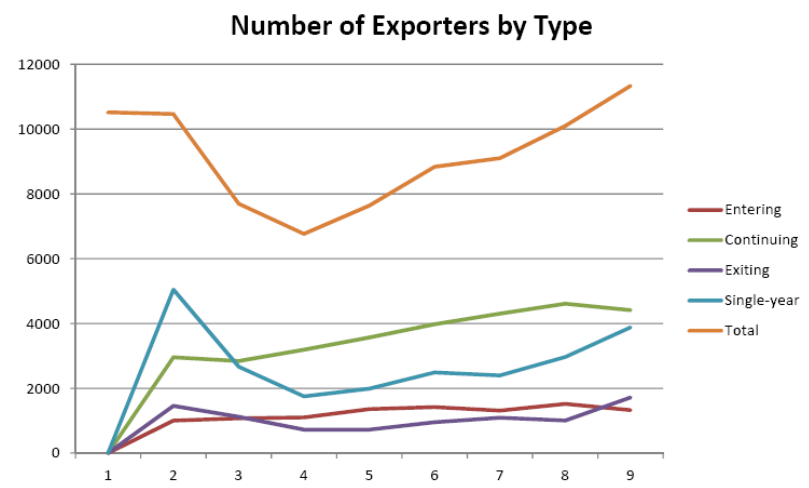
\includegraphics[
natheight=4.5074in, natwidth=7.8248in, height=1.9865in, width=3.4359in]
{figs/exp_by_type.png}%
\end{figure}%
%EndExpansion

\begin{itemize}
\item As a fraction of total exporters, firms that enter a market and
immediately exit are important.
\end{itemize}

%TCIMACRO{\TeXButton{EndFrame}{\end{frame}}}%
%BeginExpansion
\end{frame}%
%EndExpansion
%TCIMACRO{\TeXButton{BeginFrame}{\begin{frame}}}%
%BeginExpansion
\begin{frame}%
%EndExpansion

\QTR{frametitle}{Exporters by durability}

%TCIMACRO{%
%\FRAME{ftbpF}{3.3892in}{2.0851in}{0pt}{}{}{Figure}{%
%\special{language "Scientific Word";type "GRAPHIC";maintain-aspect-ratio TRUE;display "USEDEF";valid_file "T";width 3.3892in;height 2.0851in;depth 0pt;original-width 9.9955in;original-height 6.135in;cropleft "0";croptop "1";cropright "1";cropbottom "0";tempfilename 'MVUDQX01.wmf';tempfile-properties "XPR";}}}%
%BeginExpansion
\begin{figure}[ptb]\centering
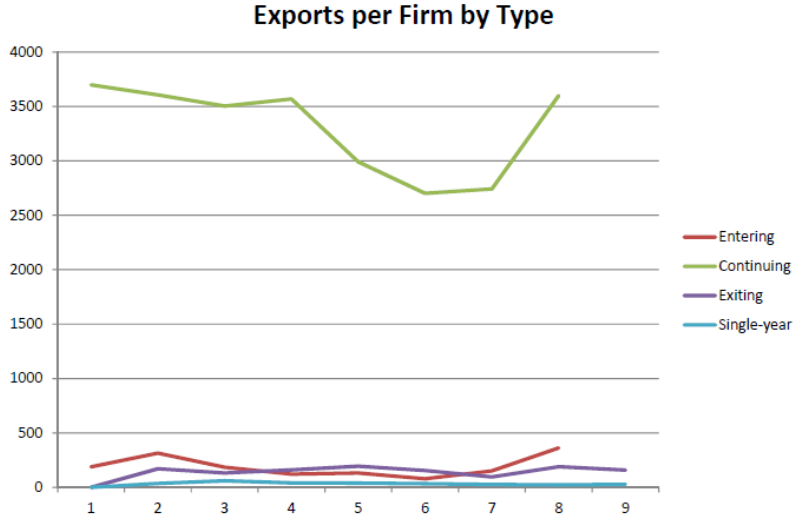
\includegraphics[
natheight=6.135in, natwidth=9.9955in, height=2.0851in, width=3.3892in]
{figs/exports_by_type.png}%
\end{figure}%
%EndExpansion

\begin{itemize}
\item But as a fraction of total export revenue, brand new exporters don't
account for much.
\end{itemize}

%TCIMACRO{\TeXButton{EndFrame}{\end{frame}}}%
%BeginExpansion
\end{frame}%
% %EndExpansion
% %TCIMACRO{\TeXButton{BeginFrame}{\begin{frame}}}%
% %BeginExpansion
\begin{frame}%
%EndExpansion

\QTR{frametitle}{Cohort maturation}

%TCIMACRO{%
%\FRAME{ftbpF}{3.3529in}{2.3514in}{0pt}{}{}{Figure}{%
%\special{language "Scientific Word";type "GRAPHIC";maintain-aspect-ratio TRUE;display "USEDEF";valid_file "T";width 3.3529in;height 2.3514in;depth 0pt;original-width 9.1618in;original-height 6.4126in;cropleft "0";croptop "1";cropright "1";cropbottom "0";tempfilename 'MVUDQX02.wmf';tempfile-properties "XPR";}}}%
%BeginExpansion
\begin{figure}[ptb]\centering
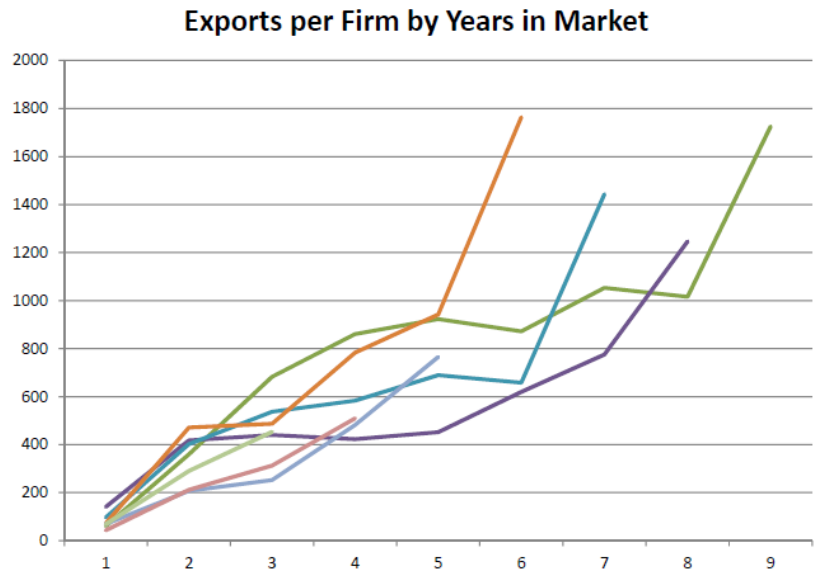
\includegraphics[
natheight=6.4126in, natwidth=9.1618in, height=2.3514in, width=3.3529in]
{figs/exp_by_coh.png}%
\end{figure}%
%EndExpansion

\begin{itemize}
\item The firms that survive their first year grow exceptionally rapidly
(see also Ruhl and Willis, 2008).
\end{itemize}

%TCIMACRO{\TeXButton{EndFrame}{\end{frame}}}%
%BeginExpansion
\end{frame}%
%EndExpansion
%TCIMACRO{\TeXButton{BeginFrame}{\begin{frame}}}%
%BeginExpansion
\begin{frame}%
%EndExpansion

\QTR{frametitle}{Cohort maturation}

%TCIMACRO{%
%\FRAME{ftbpF}{3.5717in}{2.2295in}{0pt}{}{}{Figure}{%
%\special{language "Scientific Word";type "GRAPHIC";maintain-aspect-ratio TRUE;display "USEDEF";valid_file "T";width 3.5717in;height 2.2295in;depth 0pt;original-width 9.8286in;original-height 6.1203in;cropleft "0";croptop "1";cropright "1";cropbottom "0";tempfilename 'MVUDQX03.wmf';tempfile-properties "XPR";}}}%
%BeginExpansion
\begin{figure}[ptb]\centering
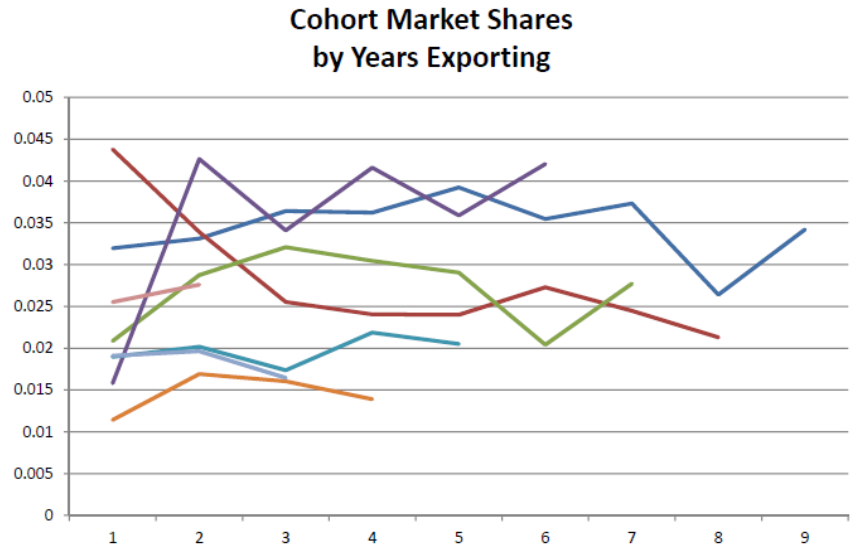
\includegraphics[
natheight=6.1203in, natwidth=9.8286in, height=2.2295in, width=3.5717in]
{figs/coh_shr.png}%
\end{figure}%
%EndExpansion

\begin{itemize}
\item Hence young cohorts typically gain market share despite rapid
attrition.

\item Post-1996 entrants account for about half of cumulative export
expansion by 2005.
\end{itemize}

%TCIMACRO{\TeXButton{EndFrame}{\end{frame}}}%
%BeginExpansion
\end{frame}%
%EndExpansion
%TCIMACRO{\TeXButton{BeginFrame}{\begin{frame}}}%
%BeginExpansion
\begin{frame}%
%EndExpansion

\QTR{frametitle}{Cohort maturation}

%TCIMACRO{%
%\FRAME{ftbpF}{3.2923in}{2.1257in}{0pt}{}{}{Figure}{%
%\special{language "Scientific Word";type "GRAPHIC";maintain-aspect-ratio TRUE;display "USEDEF";valid_file "T";width 3.2923in;height 2.1257in;depth 0pt;original-width 10.3855in;original-height 6.6902in;cropleft "0";croptop "1";cropright "1";cropbottom "0";tempfilename 'MVUDQX04.wmf';tempfile-properties "XPR";}}}%
%BeginExpansion
\begin{figure}[ptb]\centering
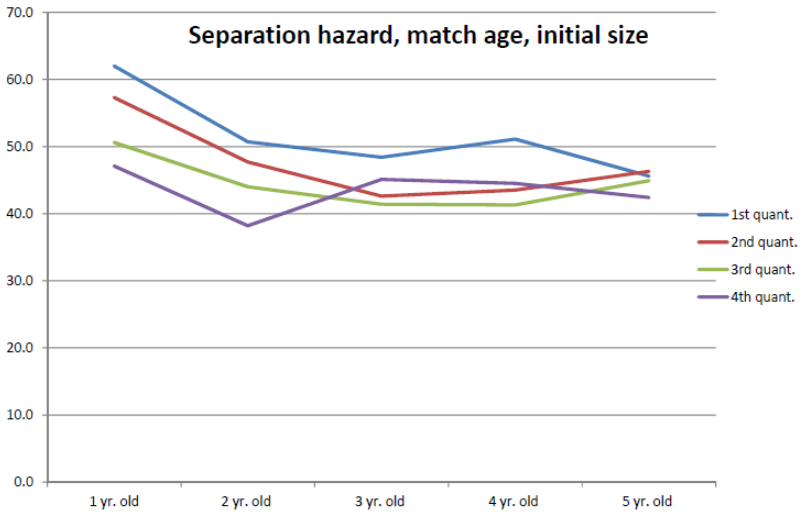
\includegraphics[
natheight=6.6902in, natwidth=10.3855in, height=2.1257in, width=3.2923in]
{figs/sep_haz.png}%
\end{figure}%
%EndExpansion

\begin{itemize}
    \item Most new matches fail within a year, but
    
    \begin{itemize}
        \item Chances of survival are higher for matches with large initial sales
        
        \item Survival rates improve and converge for all matches after the first
        year.
        
        \item To sustain or increase exports, firms must continually replenish their
        foreign clientele.
    \end{itemize}
\end{itemize}

%TCIMACRO{\TeXButton{EndFrame}{\end{frame}}}%
%BeginExpansion
\end{frame}%
%EndExpansion
%TCIMACRO{\TeXButton{BeginFrame}{\begin{frame}}}%
%BeginExpansion
\begin{frame}%
%EndExpansion

%TCIMACRO{%
%\FRAME{ftbpF}{3.5016in}{2.2969in}{0pt}{}{}{Figure}{%
%\special{language "Scientific Word";type "GRAPHIC";maintain-aspect-ratio TRUE;display "USEDEF";valid_file "T";width 3.5016in;height 2.2969in;depth 0pt;original-width 12.276in;original-height 8.0367in;cropleft "0";croptop "1";cropright "1";cropbottom "0";tempfilename 'MVUDQX05.wmf';tempfile-properties "XPR";}}}%
%BeginExpansion
\begin{figure}[ptb]\centering
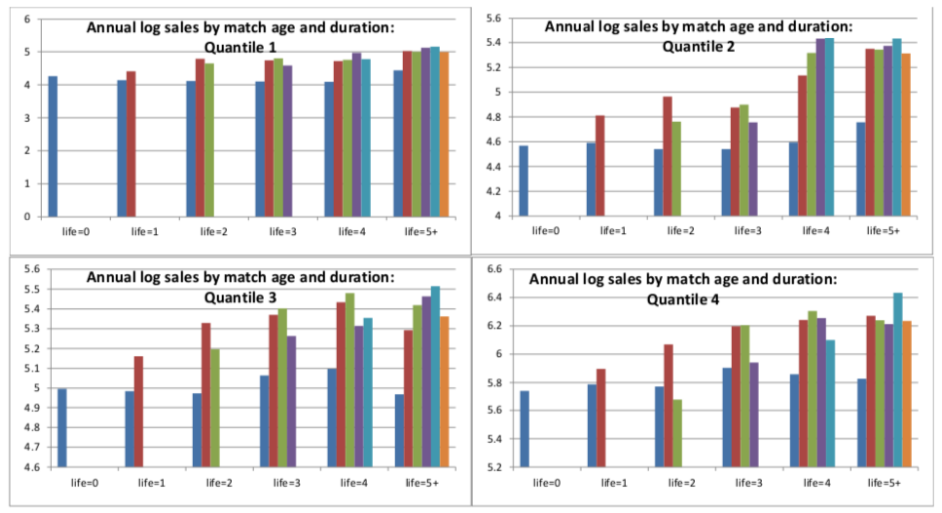
\includegraphics[
natheight=8.0367in, natwidth=12.276in, height=2.2969in, width=3.5016in]
{figs/match_dyn.png}%
\end{figure}%
%EndExpansion
\bigskip

\begin{itemize}
\item Matches that start small tend to stay small.

\item After a match's first year, there is no systematic tendency for its
annual sales to grow.
\end{itemize}

%TCIMACRO{\TeXButton{EndFrame}{\end{frame}}}%
%BeginExpansion
\end{frame}%
%EndExpansion
%TCIMACRO{\TeXButton{BeginFrame}{\begin{frame}}}%
%BeginExpansion

\begin{frame}{Power-law distributions}

    \begin{itemize} 
        \item A distribution $G(x)$ is \textbf{power law} if its right-tail is distributed Pareto:
            \begin{equation}
                F_{\mbox{{\tiny{Pareto}}}}(x;\theta,x_{\tiny\mbox{min}}) = 1 - \left(\frac{x}{x_{\tiny\mbox{min}}}\right)^{-\theta} \nonumber
            \end{equation}
        \item The log of $1 - F_{\mbox{{\tiny{Pareto}}}}$ is a linear function of $\log{x}$:
            \begin{equation}
                \log\left({1 - F_{\mbox{\tiny{Pareto}}}(x;\theta,x_{\tiny\mbox{min}})}\right) = -\theta \log{x} + C\nonumber
            \end{equation}
        \item If data are distributed power law, a scatter plot of the log empirical inverse CDF and log of the data will be linear in the tail ($\approx$ Gibrat's law)
        \item If data are distributed Pareto, a scatter plot of the log empirical inverse CDF and log of the data will be linear everywhere (Zipf's law)
    \end{itemize}

\end{frame}

\begin{frame}%
%EndExpansion

\QTR{frametitle}{A seriously Pareto client distribution}

\begin{itemize}
\item Most firms have a single buyer, but the distribution of client counts
across exporters is fat-tailed.

%TCIMACRO{%
%\FRAME{ftbpF}{3.4817in}{2.5694in}{0pt}{}{}{Figure}{%
%\special{language "Scientific Word";type "GRAPHIC";maintain-aspect-ratio TRUE;display "USEDEF";valid_file "T";width 3.4817in;height 2.5694in;depth 0pt;original-width 11.6637in;original-height 8.591in;cropleft "0";croptop "1";cropright "1";cropbottom "0";tempfilename 'MVUDQX06.wmf';tempfile-properties "XPR";}}}%
%BeginExpansion
\begin{figure}[ptb]\centering
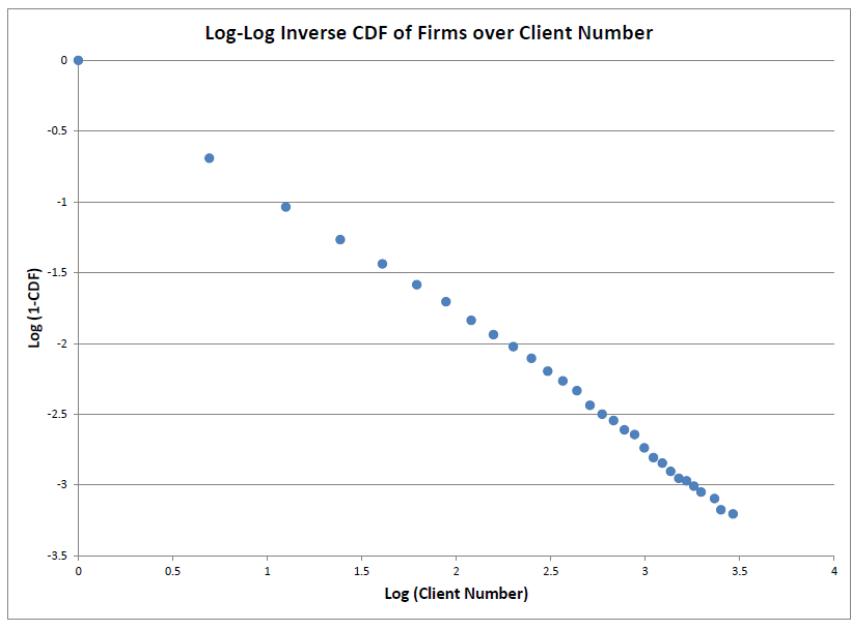
\includegraphics[
natheight=8.591in, natwidth=11.6637in, height=2.5694in, width=3.4817in]
{figs/fat_tail.png}%
\end{figure}%
%EndExpansion
\end{itemize}

%TCIMACRO{\TeXButton{EndFrame}{\end{frame}}}%
%BeginExpansion
\end{frame}%
%EndExpansion
%TCIMACRO{\TeXButton{BeginFrame}{\begin{frame}}}%
%BeginExpansion
\begin{frame}%
%EndExpansion

\QTR{frametitle}{Year-to-year transitions in numbers of clients}

\begin{tabular}{llllllllll}
\multicolumn{10}{c}{\small Table 3: Transition Probabilities, Number of
Clients} \\ \hline\hline
{\small t}$\backslash ${\small t+1} & {\small exit} & {\small texit} & 
{\small 1} & {\small 2} & {\small 3} & {\small 4} & {\small 5} & {\small 6-10%
} & {\small 11+} \\ \hline
{\small enter} & {\small 0.000} & {\small 0.000} & {\small 0.947} & {\small %
0.044} & {\small 0.007} & {\small 0.002} & {\small 0.001} & {\small 0.001} & 
{\small 0.000} \\ 
{\small texit} & {\small 0.000} & {\small .} & {\small 0.896} & {\small 0.086%
} & {\small 0.014} & {\small 0.004} & {\small .} & {\small .} & {\small 0.000%
} \\ 
{\small 1} & {\small 0.533} & {\small 0.081} & {\small 0.332} & {\small 0.043%
} & {\small 0.008} & {\small 0.002} & {\small 0.001} & {\small .} & {\small .%
} \\ 
{\small 2} & {\small 0.180} & {\small 0.081} & {\small 0.375} & {\small 0.249%
} & {\small 0.077} & {\small 0.026} & {\small 0.007} & {\small 0.005} & 
{\small 0.000} \\ 
{\small 3} & {\small 0.074} & {\small 0.043} & {\small 0.225} & {\small 0.282%
} & {\small 0.206} & {\small 0.093} & {\small 0.047} & {\small .} & {\small .%
} \\ 
{\small 4} & {\small 0.045} & {\small .} & {\small 0.112} & {\small 0.226} & 
{\small 0.259} & {\small 0.162} & {\small 0.097} & {\small 0.078} & {\small .%
} \\ 
{\small 5} & {\small .} & {\small .} & {\small 0.103} & {\small 0.184} & 
{\small 0.197} & {\small 0.184} & {\small 0.094} & {\small 0.197} & {\small .%
} \\ 
{\small 6-10} & {\small .} & {\small .} & {\small .} & {\small 0.070} & 
{\small 0.082} & {\small 0.114} & {\small 0.149} & {\small 0.465} & {\small %
0.066} \\ 
{\small 11+} & {\small 0.000} & {\small 0.000} & {\small 0.000} & {\small %
0.000} & {\small 0.000} & {\small .} & {\small .} & {\small 0.440} & {\small %
0.460} \\ \hline
\end{tabular}%
{\small \ }

%TCIMACRO{\TeXButton{EndFrame}{\end{frame}}}%
%BeginExpansion
\end{frame}%
%EndExpansion
%TCIMACRO{\TeXButton{BeginFrame}{\begin{frame}}}%
%BeginExpansion
\begin{frame}%
%EndExpansion

\QTR{frametitle}{Key model features}

\begin{itemize}
\item Firms engage in costly \textbf{search} to meet potential buyers at
home and (possibly) abroad.

\item Firms new to the foreign market don't know what fraction of buyers
there will be willing to do business with them.

\item As they encounter potential buyers, firms gradually learn the scope of
the market for their particular products, and they adjust their search
intensities accordingly (\textbf{learning}).

\item Search costs fall as firms accumulate successful business
relationships \textbf{(reputation effects}).

\item Maintaining a relationship with a buyer is costly, so a relationship
that yields meager profits is dropped.

\item Three types of shocks: marketwide, firm-specific, match-specific
\end{itemize}

%TCIMACRO{\TeXButton{EndFrame}{\end{frame}}}%
%BeginExpansion
\end{frame}%
%EndExpansion
%TCIMACRO{\TeXButton{BeginFrame}{\begin{frame}}}%
%BeginExpansion
\begin{frame}%
%EndExpansion

\QTR{frametitle}{Three model components}

\begin{enumerate}
\item A Seller-Buyer Relationship

\item Learning About Product Appeal from Encounters with Potential Buyers

\item Searching for Potential Buyers
\end{enumerate}

%TCIMACRO{\TeXButton{EndFrame}{\end{frame}}}%
%BeginExpansion
\end{frame}%
%EndExpansion
%TCIMACRO{\TeXButton{BeginFrame}{\begin{frame}}}%
%BeginExpansion
\begin{frame}%
%EndExpansion

\QTR{frametitle}{Why continuous time?}

\begin{itemize}
\item Two types of discrete events occur at random intervals, sometimes with
high frequency

\begin{itemize}
\item Sellers meet buyers

\item Once business relationships are established, orders are placed
\end{itemize}

\item With continuous time formulation we can:

\begin{itemize}
\item allow for an arbitrarily large number of events during any discrete
interval

\item allow agents to update their behavior each time an event occurs
\end{itemize}
\end{itemize}

%TCIMACRO{\TeXButton{EndFrame}{\end{frame}}}%
%BeginExpansion
\end{frame}%
%EndExpansion
%TCIMACRO{\TeXButton{BeginFrame}{\begin{frame}}}%
%BeginExpansion
\begin{frame}%
%EndExpansion

\QTR{frametitle}{1. Relationship dynamics}

\QTR{framesubtitle}{profits from a shipment}

\begin{itemize}
\item Define exogenous state variables:

\begin{itemize}
\item $\varphi _{j}$ productivity of seller $j$

\item $x_{t}^{m}$ size of market $m\in \left\{ h,f\right\} $ (Markov jump
process)

\item $y_{ijt}^{m}$ idiosyncratic shock to operating profits from shipment
to buyer $i$ by seller $j$ in market $m$ (Markov jump process)

\item $\Pi ^{m}$ profit function scalar (so that all exogenous state
variables can be normalized to mean log zero)
\end{itemize}

\item When buyer $i$ places an order with seller $j$ in market $m$ it
generates operating profits:%
\[
\pi (x_{t}^{m},\varphi _{j},y_{ijt}^{m})=\Pi ^{m}x_{t}^{m}\varphi
_{j}^{\sigma -1}y_{ijt}^{m}. 
\]
\end{itemize}

Superscripts and subcripts mostly suppressed hereafter:%
\[
\pi _{\varphi }(x,y)=\Pi x\varphi ^{\eta -1}y 
\]

%TCIMACRO{\TeXButton{EndFrame}{\end{frame}}}%
%BeginExpansion
\end{frame}%
%EndExpansion
%TCIMACRO{\TeXButton{BeginFrame}{\begin{frame}}}%
%BeginExpansion
\begin{frame}%
%EndExpansion

\QTR{frametitle}{1. Relationship dynamics}

\QTR{framesubtitle}{value of a business relationship}

\begin{itemize}
\item In active business relationships, buyers place orders with exogenous
hazard $\lambda ^{b}$.%
%TCIMACRO{\qhyperref{}{}{appendix}{\beamergotobutton{Details}}}%
%BeginExpansion
\hyperref{}{}{appendix}{\beamergotobutton{Details}}%
%EndExpansion

\item After each order, sellers must pay fixed cost $F$ to keep a business
relationship active.

\item Value to a type-$\varphi $ seller of a relationship in state $\{x,y\}$:%
\[
\widetilde{\pi }_{\varphi }(x,y)=\pi _{\varphi }(x,y)+\max \left\{ \widehat{%
\pi }_{\varphi }(x,y)-F,0\right\} 
\]

\item $\widehat{\pi }_{\varphi }(x,y)$ is continuation value to a type-$%
\varphi $ seller of a relationship in state $\{x,y\}$ 
%TCIMACRO{\qhyperref{}{}{pihat_derivation}{\beamergotobutton{Details}}}%
%BeginExpansion
\hyperref{}{}{pihat_derivation}{\beamergotobutton{Details}}%
%EndExpansion
.

\item Continuation values depend negatively on

\begin{itemize}
\item $\delta :$ exogenous hazard of relationship death.

\item $\rho :$ seller's discount rate (including exogenous seller death probability)
\end{itemize}
\end{itemize}

%TCIMACRO{\TeXButton{EndFrame}{\end{frame}}}%
%BeginExpansion
\end{frame}%
%EndExpansion
%TCIMACRO{\TeXButton{BeginFrame}{\begin{frame}}}%
%BeginExpansion
\begin{frame}%
%EndExpansion

\QTR{frametitle}{1. Relationship dynamics}

\QTR{framesubtitle}{expected value of a new relationship}

\begin{itemize}
\item Sellers don't know what $y$ value their next business relationship
will begin from.

\item Let $\Pr (y^{s})$ be the probability of initial shock $y^{s}$
determined by the ergodic distribution of $y$.

\item Expected value of a successful new encounter:%
\[
\widetilde{\pi }_{\varphi }(x)=\sum_{y^{s}}\Pr (y^{s})\widetilde{\pi }%
_{\varphi }(x,y) 
\]
\end{itemize}

%TCIMACRO{\TeXButton{EndFrame}{\end{frame}}}%
%BeginExpansion
\end{frame}%
%EndExpansion
%TCIMACRO{\TeXButton{BeginFrame}{\begin{frame}}}%
%BeginExpansion
\begin{frame}%
%EndExpansion

\QTR{frametitle}{2. Learning about product appeal}

\QTR{framesubtitle}{the "true" scope of the market}

\begin{itemize}
\item Fraction of potential buyers in market $m$ who are interested in
seller $j$'s product: $\theta _{j}^{m}\in \lbrack 0,1]$ of total potential
buyers.

\item Assume $\theta _{j}^{^{m}\prime }s$ are time-invariant, mutually
independent draws from a beta distribution:
\end{itemize}

\[
r(\theta |\alpha ,\beta )=\frac{\Gamma (\alpha +\beta )}{\Gamma (\alpha
)\Gamma (\beta )}\left( \theta \right) ^{\alpha -1}(1-\theta )^{\beta -1}, 
\]

\begin{itemize}
\item Expected value:%
\[
E(\theta |\alpha ,\beta )=\frac{\alpha }{\alpha +\beta .} 
\]

\item Posterior beliefs, after meeting $n^{m}$ potential clients in market $%
m $, $a^{m}$ of whom want to do business:%
%TCIMACRO{\qhyperref{}{}{Bayesian_details}{\beamergotobutton{Details}}}%
%BeginExpansion
\hyperref{}{}{Bayesian_details}{\beamergotobutton{Details}}%
%EndExpansion
\[
\overline{\theta }^{m}(a^{m},n^{m})=E\left[ \theta ^{m}|a^{m},n^{m}\right] =%
\frac{a^{m}+\alpha }{n^{m}+\alpha +\beta } 
\]
\end{itemize}

%TCIMACRO{\TeXButton{EndFrame}{\end{frame}}}%
%BeginExpansion
\end{frame}%
%EndExpansion
%TCIMACRO{\TeXButton{BeginFrame}{\begin{frame}}}%
%BeginExpansion
\begin{frame}%
%EndExpansion

\QTR{frametitle}{3. Searching for buyers}

\QTR{framesubtitle}{the cost of search}

\begin{itemize}
\item Seller continuously chooses the hazard $s$ with which she encounters a
potential buyer at a flow cost $c(s,a)$

\begin{itemize}
\item Maintain web site

\item Pay to be near top of web search listings

\item Attend trade fairs

\item Research foreign buyers

\item Send sales reps. to foreign markets

\item Maintain foreign sales office
\end{itemize}

\item The number of successful encounters, $a$, allows for network effects
(NYT 2/27/12: Panjiva, ImportGenius).

\item Functional form used for estimation (Arkolakis, 2010):%
\[
c(s,a)=\kappa _{0}\frac{(1+s)^{\left( 1+1/\kappa _{1}\right) }-1}{%
(1+a)^{\gamma \cdot \left( 1+1/\kappa _{1}\right) }\left( 1+1/\kappa
_{1}\right) } 
\]
\end{itemize}

%TCIMACRO{\TeXButton{EndFrame}{\end{frame}}}%
%BeginExpansion
\end{frame}%
%EndExpansion
%TCIMACRO{\TeXButton{BeginFrame}{\begin{frame}}}%
%BeginExpansion
\begin{frame}%
%EndExpansion

\QTR{frametitle}{3. Searching for buyers}

\QTR{framesubtitle}{the value of search abroad}

\begin{itemize}
\item Let $V_{\varphi }(a,n,x)$ be the value of continued search for a type-$%
\varphi $ firm with $a$ successes in $n$ meetings.

\item The first-order for optimal search abroad is:%
%TCIMACRO{\qhyperref{}{}{optimal_search}{\beamergotobutton{Details}}}%
%BeginExpansion
\hyperref{}{}{optimal_search}{\beamergotobutton{Details}}%
%EndExpansion
\begin{eqnarray*}
c_{s}(s^{\ast },a) &=&\overline{\theta }_{a,n}(\widetilde{\pi }_{\varphi
}(x)+V_{\varphi }(a+1,n+1,x)) \\
&&+(1-\overline{\theta }_{a,n})V_{\varphi }(a,n+1,x)-V_{\varphi }(a,n,x).
\end{eqnarray*}
\end{itemize}

%TCIMACRO{\TeXButton{EndFrame}{\end{frame}}}%
%BeginExpansion
\end{frame}%
%EndExpansion
%TCIMACRO{\TeXButton{BeginFrame}{\begin{frame}}}%
%BeginExpansion
\begin{frame}%
%EndExpansion

\QTR{frametitle}{3. Searching for buyers}

\QTR{framesubtitle}{when the truth is known: the domestic market}

\begin{itemize}
\item As $n$ increases $\overline{\theta }_{a,n}$ converges to the true $%
\theta .$ There is no more learning and the reward to search depends on $a$
and $n$ only through network effects.

\item We assume this characterizes the domestic market, so the first-order
condition for optimal search at home is:%
\[
c_{s}(s^{\ast },a)=\theta _{j}\widetilde{\pi }_{\varphi }(x). 
\]
\end{itemize}

%TCIMACRO{\TeXButton{EndFrame}{\end{frame}}}%
%BeginExpansion
\end{frame}%
%EndExpansion
%TCIMACRO{\TeXButton{BeginFrame}{\begin{frame}}}%
%BeginExpansion
\begin{frame}%
%EndExpansion

\begin{flushleft}
\QTR{frametitle}{Estimation}

\QTR{framesubtitle}{The exogenous state variables}
\end{flushleft}

\begin{itemize}
\item Assume $x^{f},$ $x^{h},$ and $y$ follow independent Ehrenfest
diffusion processes.

\begin{itemize}
\item Any variable $z$ that obeys this process is discretized into $2e+1$
possible values, $e\in I^{+}:$ $z\in \{-e\Delta ,$ $-(e-1)\Delta ,$ $..,$ $%
0,..,$ $(e-1)\Delta ,$ $e\Delta \}.$

\item Process jumps with hazard $\lambda _{z},$ and when it does so:%
\[
z^{\prime }=\left\{ 
\begin{array}{c}
z+\Delta \\ 
z-\Delta \\ 
\text{other}%
\end{array}%
\right. \text{with probability }\left\{ 
\begin{array}{c}
\frac{1}{2}\left( 1-\frac{z}{e\bigtriangleup }\right) \\ 
\frac{1}{2}\left( 1+\frac{z}{e\bigtriangleup }\right) \\ 
0%
\end{array}%
\right. . 
\]
\end{itemize}

\item As the grid becomes finer, this type of random variable asymptotes to
an Ornstein-Uhlenbeck processes: 
\[
dz=-\mu zdt+\sigma dW 
\]
\end{itemize}

%TCIMACRO{\TeXButton{EndFrame}{\end{frame}}}%
%BeginExpansion
\end{frame}%
%EndExpansion
%TCIMACRO{\TeXButton{BeginFrame}{\begin{frame}}}%
%BeginExpansion
\begin{frame}%
%EndExpansion

\begin{flushleft}
\QTR{frametitle}{Estimation}

\QTR{framesubtitle}{The exogenous state variables}
\end{flushleft}

\begin{itemize}
\item If $z$ observed at regular intervals, can estimate $\mu $ and $\sigma $
by regressing $z$ on lagged $z$

\item For $x^{f},x^{h},$ obtain maximum likelihood estimates of $\mu $ and $%
\sigma $ using logged and de-meaned time series on total real consumption of
manufactured goods in each country.

\item Recover $\lambda _{z}$ and $\Delta $ using Shimer's result that
asymptotically, $\mu =\lambda _{z}/e$, $\sigma =\sqrt{\lambda _{z}}\Delta $.

\item This gives us the $q_{xx^{\prime }}^{X}$ values needed to construct $%
q_{yy^{\prime }}^{Y}$'s for home and foreign markets.

\item Since $y$ is unobservable, recover the parameters of its jump
processes using the structure of the dynamic model.
\end{itemize}

%TCIMACRO{\TeXButton{EndFrame}{\end{frame}}}%
%BeginExpansion
\end{frame}%
%EndExpansion
%TCIMACRO{\TeXButton{BeginFrame}{\begin{frame}}}%
%BeginExpansion
\begin{frame}%
%EndExpansion

\begin{flushleft}
\QTR{frametitle}{Estimation}

\QTR{framesubtitle}{The exogenous state variables}
\end{flushleft}

\begin{center}
\begin{tabular}{lcc}
\hline\hline
\multicolumn{3}{c}{\textbf{Market-wide Shock Processes (}$x^{f},x^{h}$%
\textbf{)}} \\ \hline
\textbf{Orstein-Uhlenbeck Parameters} & \textbf{Colombia} & \textbf{United
States} \\ \hline
$\mu ${\small \ Mean Reversion} & {\small 0.171} & {\small 0.174} \\ 
$\sigma ${\small \ Dispersion} & {\small 0.003} & {\small 0.058} \\ \hline
\textbf{Ehrenfest Process Parameters} &  &  \\ \hline
$\lambda ${\small \ Jump Hazard} & {\small 1.200} & {\small 1.215} \\ 
$\Delta ${\small \ Jump Size} & {\small 0.003} & {\small 0.053} \\ 
{\small grid points} & {\small 15} & {\small 15} \\ \hline
\end{tabular}
\end{center}

%TCIMACRO{\TeXButton{EndFrame}{\end{frame}}}%
%BeginExpansion
\end{frame}%
%EndExpansion
%TCIMACRO{\TeXButton{BeginFrame}{\begin{frame}}}%
%BeginExpansion
\begin{frame}%
%EndExpansion

\QTR{frametitle}{Estimation}

\QTR{framesubtitle}{remaining parameters}

\begin{itemize}
\item Unidentified preference parameters taken from literature: Discount rate (including 0.03 exogenous death) $\rho =0.05,$ Demand elasticity $\sigma =5$

\item Remaining parameters identified using indirect inference
\end{itemize}

\[
\Lambda =\left( {\small \Pi }^{h},{\small \Pi }^{f},{\small \delta ,}F,%
{\small \alpha },{\small \beta },\sigma _{\varphi },\lambda _{y},\Delta_{y},{\small %
\lambda }_{b},{\small \gamma ,\kappa _{0},\kappa _{1}}\right) 
\]

%TCIMACRO{\TeXButton{EndFrame}{\end{frame}}}%
%BeginExpansion
\end{frame}%
%EndExpansion
%TCIMACRO{\TeXButton{BeginFrame}{\begin{frame}}}%
%BeginExpansion
\begin{frame}%
%EndExpansion

\QTR{frametitle}{Indirect inference (Gouri\'{e}roux and Monfort, 1996)}

\QTR{framesubtitle}{basic idea}

\begin{itemize}
\item Using reduced-form auxillary regressions and/or moments, summarize key
relationships in the data using a vector of statistics ($\widehat{\mathbf{M}}
$)

\item Similar to Simulated Method of Moments -- difference is a bit philosophical 

\item For a candidate set of parameter values ($\Lambda $), simulate same
statistics using the model $\widehat{\mathbf{M}}^{s}$($\Lambda $).

\item Construct the loss function: 
\[
Q(\Lambda )=\left( \widehat{\mathbf{M}}-\widehat{\mathbf{M}}^{s}(\Lambda
)\right) ^{\prime }\Omega \left( \widehat{\mathbf{M}}-\widehat{\mathbf{M}}%
^{s}(\Lambda )\right) 
\]%
where $\Omega $ is a positive definite weighting matrix.

\item Use a robust algorithm to search parameter space for $\widehat{\Lambda 
}=\arg \min Q(\Lambda ).$
\end{itemize}

%TCIMACRO{\TeXButton{EndFrame}{\end{frame}}}%
%BeginExpansion
\end{frame}%
%EndExpansion
%TCIMACRO{\TeXButton{BeginFrame}{\begin{frame}}}%
%BeginExpansion
\begin{frame}%
%EndExpansion

\QTR{frametitle}{Indirect inference}

\QTR{framesubtitle}{identification}

\begin{itemize}
\item \textbf{Profit scaling constants}, (${\small \Pi }^{h}$, ${\small \Pi }%
^{f})$

\begin{itemize}
\item means of log home and foreign sales
\end{itemize}

\item \textbf{Shipment hazards} (${\small \lambda }^{b}$)

\begin{itemize}
\item average annual shipment rates per match
\end{itemize}

\item \textbf{Product appeal parameters} $(\alpha ,$\ $\beta )$

\begin{itemize}
\item distribution of home and foreign sales
\end{itemize}

\item \textbf{Firm productivity dispersion} $(\sigma _{\varphi })$

\begin{itemize}
\item covariance of home and foreign sales
\end{itemize}

\item \textbf{Search cost parameters} (${\small \kappa }_{0}{\small ,}$ $%
\kappa _{1},$ $\gamma )$

\begin{itemize}
\item match rates

\item client frequency distribution (especially fatness of tail)

\item client transition probabilites

\item fraction of firms that export
\end{itemize}
\end{itemize}

%TCIMACRO{\TeXButton{EndFrame}{\end{frame}}}%
%BeginExpansion
\end{frame}%
%EndExpansion
%TCIMACRO{\TeXButton{BeginFrame}{\begin{frame}}}%
%BeginExpansion
\begin{frame}%
%EndExpansion

\QTR{frametitle}{Indirect inference}

\QTR{framesubtitle}{identification}

\begin{itemize}
    \item \textbf{Idioysncratic shocks to importers (}$\lambda ^{y}$, $\Delta^{y}$\textbf{)}

\begin{itemize}
\item cross-plant variances in home and foreign sales

\item covariation of home and foreign sales

\item autocorrelation, match-specific sales

\item client frequency distribution, client transition probabilites
\end{itemize}

\item \textbf{Match maintenance costs} (${\small F)}$

\begin{itemize}
\item client frequency distribution, client transition probabilites

\item sales among new versus established matches

\item age-specific match failure rates
\end{itemize}

\item \textbf{Exogenous match separation hazard} (${\small \delta }{\small )}
$

\begin{itemize}
\item separation rates after first year

\item age-specific match failure rates

\item client frequency distribution
\end{itemize}
\end{itemize}

%TCIMACRO{\TeXButton{EndFrame}{\end{frame}}}%
%BeginExpansion
\end{frame}%
%EndExpansion
%TCIMACRO{\TeXButton{BeginFrame}{\begin{frame}}}%
% %BeginExpansion
\begin{frame}%
%EndExpansion

\QTR{frametitle}{Data versus simulated statistics}

\begin{center}
{\small 
\begin{tabular}{llllll}
\multicolumn{6}{c}{} \\ \hline\hline
\textbf{Transition probs., }                   &                           &                           & \textbf{Share of firms }        &                            &                           \\
\textbf{no. clients (}$n^{c}$\textbf{)}        & \multicolumn{1}{r}{Data}  & \multicolumn{1}{r}{Model} & \textbf{exporting}              & \multicolumn{1}{r}{Data}   & \multicolumn{1}{r}{Model} \\ \hline
$\widehat{P}[n_{jt+1}^{c}=0|n_{jt}^{c}=1]$     & \multicolumn{1}{r}{0.618} & \multicolumn{1}{r}{0.650} & $\widehat{E}(1_{X_{jt}^{f}>0})$ & \multicolumn{1}{r}{0.299}  & \multicolumn{1}{r}{0.359} \\
$\widehat{P}[n_{jt+1}^{c}=1|n_{jt}^{c}=1]$     & \multicolumn{1}{r}{0.321} & \multicolumn{1}{r}{0.320} &                                 & \multicolumn{1}{r}{}       & \multicolumn{1}{r}{}      \\
$\widehat{P}[n_{jt+1}^{c}=2|n_{jt}^{c}=1]$     & \multicolumn{1}{r}{0.048} & \multicolumn{1}{r}{0.027} & \textbf{Log foreign sales on}   & \multicolumn{1}{r}{}       & \multicolumn{1}{r}{}      \\
$\widehat{P}[n_{jt+1}^{c}\geq 3|n_{jt}^{c}=1]$ & \multicolumn{1}{r}{0.013} & \multicolumn{1}{r}{0.002} & \textbf{log domestic sales}     & \multicolumn{1}{r}{ Data}  & \multicolumn{1}{r}{Model} \\ \cline{4-6}
$\widehat{P}[n_{jt+1}^{c}=0|n_{jt}^{c}=2]$     & \multicolumn{1}{r}{0.271} & \multicolumn{1}{r}{0.443} &                                 & \multicolumn{1}{r}{}       & \multicolumn{1}{r}{}      \\
$\widehat{P}[n_{jt+1}^{c}=1|n_{jt}^{c}=2]$     & \multicolumn{1}{r}{0.375} & \multicolumn{1}{r}{0.339} & $\widehat{\beta }_{1}^{hf}$     & \multicolumn{1}{r}{ 0.727} & \multicolumn{1}{r}{0.877} \\
$\widehat{P}[n_{jt+1}^{c}=2|n_{jt}^{c}=2]$     & \multicolumn{1}{r}{0.241} & \multicolumn{1}{r}{0.165} & $s\widehat{e}(\epsilon ^{hf})$  & \multicolumn{1}{r}{2.167}  & \multicolumn{1}{r}{0.640} \\
$\widehat{P}[n_{jt+1}^{c}\geq 3|n_{jt}^{c}=2]$ & \multicolumn{1}{r}{0.113} & \multicolumn{1}{r}{0.052} &                                 & \multicolumn{1}{r}{}       & \multicolumn{1}{r}{}      \\ \hline
\end{tabular}%
}
\end{center}

%TCIMACRO{\TeXButton{EndFrame}{\end{frame}}}%
%BeginExpansion
\end{frame}%
% %EndExpansion
% %TCIMACRO{\TeXButton{BeginFrame}{\begin{frame}}}%
% %BeginExpansion
\begin{frame}%
%EndExpansion

\QTR{frametitle}{Data versus simulated statistics}

\begin{center}
{\small 
\begin{tabular}{lrrlrr}
\multicolumn{6}{c}{} \\ \hline\hline
\textbf{Match death hazards}      & Data  & Model & \textbf{Exporter exit rate}       & Data  & Model \\ \hline
$Death$ $rate,$ $A_{ijt-1}^{m}=0$ & 0.694 & 0.649 & $Exit$ $rate,$ $ A_{ijt-1}^{m}=0$ & 0.709 & 0.725 \\
$Death$ $rate,$ $A_{ijt-1}^{m}=1$ & 0.515 & 0.484 & $Exit$ $rate,$ $ A_{ijt-1}^{m}=1$ & 0.383 & 0.312 \\
$Death$ $rate,$ $A_{ijt-1}^{m}=2$ & 0.450 & 0.531 & $Exit$ $rate,$ $ A_{ijt-1}^{m}=2$ & 0.300 & 0.462 \\
$Death$ $rate,$ $A_{ijt-1}^{m}=3$ & 0.424 & 0.546 & $Exit$ $rate,$ $ A_{ijt-1}^{m}=3$ & 0.263 & 0.102 \\
$Death$ $rate,$ $A_{ijt-1}^{m}=4$ & 0.389 & 0.485 & $Exit$ $rate,$ $ A_{ijt-1}^{m}=4$ & 0.293 & 0.200 \\ \hline
\end{tabular}%
}
\end{center}

%TCIMACRO{\TeXButton{EndFrame}{\end{frame}}}%
%BeginExpansion
\end{frame}%
%EndExpansion
%TCIMACRO{\TeXButton{BeginFrame}{\begin{frame}}}%
%BeginExpansion
\begin{frame}%
%EndExpansion

\QTR{frametitle}{Data versus simulated statistics}

\begin{center}
{\small 
\begin{tabular}{llllll}
\multicolumn{6}{c}{} \\ \hline\hline
\textbf{Log sales per client }    &                            &                             & \textbf{Ave. log \ sales}                      &                             &                            \\
\textbf{vs. no. clients}          & \multicolumn{1}{r}{Data}   & \multicolumn{1}{r}{ Model}  & \textbf{\ by cohort age }                      & \multicolumn{1}{r}{Data}    & \multicolumn{1}{r}{Model}  \\ \hline
$\widehat{\beta }_{1}^{m}$        & \multicolumn{1}{r}{2.677}  & \multicolumn{1}{r}{0.422}   & $\widehat{E}(\ln X_{jt}^{f}|A_{jt}^{c}=0)$     & \multicolumn{1}{r}{ 8.960}  & \multicolumn{1}{r}{10.181} \\
$\widehat{\beta }_{2}^{m}$        & \multicolumn{1}{r}{-0.143} & \multicolumn{1}{r}{0.317}   & $\widehat{E}(\ln X_{jt}^{f}|A_{jt}^{c}=1)$     & \multicolumn{1}{r}{ 10.018} & \multicolumn{1}{r}{11.124} \\
$s\widehat{e}(\epsilon ^{m})$     & \multicolumn{1}{r}{2.180}  & \multicolumn{1}{r}{1.449}   & $\widehat{E}(\ln X_{jt}^{f}|A_{jt}^{c}=2)$     & \multicolumn{1}{r}{10.231}  & \multicolumn{1}{r}{11.030} \\
\textbf{No. clients, inverse}     & \multicolumn{1}{r}{}       & \multicolumn{1}{r}{}        & $\widehat{E}(\ln X_{jt}^{f}|A_{jt}^{c}=3)$     & \multicolumn{1}{r}{10.369}  & \multicolumn{1}{r}{11.021} \\
\textbf{CDF regression}           & \multicolumn{1}{r}{Data}   & \multicolumn{1}{r}{Model }  & $\widehat{E}(\ln X_{jt}^{f}|A_{jt}^{c}\geq 4)$ & \multicolumn{1}{r}{ 10.473} & \multicolumn{1}{r}{11.178} \\ \cline{1-3}
$\widehat{\beta _{1}}^{c}$        & \multicolumn{1}{r}{-1.667} & \multicolumn{1}{r}{ -2.501} &                                                & \multicolumn{1}{r}{}        & \multicolumn{1}{r}{}       \\
$s\widehat{e}(\epsilon ^{n^{c}})$ & \multicolumn{1}{r}{0.066}  & \multicolumn{1}{r}{  0.048} &                                                & \multicolumn{1}{r}{}        & \multicolumn{1}{r}{}       \\
                                  &                            &                             &                                                & \multicolumn{1}{r}{}        & \multicolumn{1}{r}{}       \\ \hline
\end{tabular}%
}{\tiny \ }
\end{center}

%TCIMACRO{\TeXButton{EndFrame}{\end{frame}}}%
%BeginExpansion
\end{frame}%
%EndExpansion
%TCIMACRO{\TeXButton{BeginFrame}{\begin{frame}}}%
%BeginExpansion
\begin{frame}%
%EndExpansion

\QTR{frametitle}{Data versus simulated statistics}

\begin{center}
{\small 
\begin{tabular}{lrrlrr}
 \multicolumn{6}{c}{} \\ \hline\hline
\textbf{Match death }                    &        &        & $\ $\textbf{Log match }          &       &       \\
\textbf{prob regression}                 & Data   & Model  & $\ $\textbf{sale autoreg.}       & Data  & Model \\ \hline
$\widehat{\beta }_{0}^{d}$               & 1.174  & 1.277  & $\widehat{\beta }_{1}^{f}$       & 0.811 & 0.849 \\
$\widehat{\beta }_{\mbox{1st year}}^{d}$ & 0.166  & 0.061  & $\beta _{\mbox{1st year}}^{f}$ & 0.233 & 0.150 \\
$\widehat{\beta }_{\mbox{lsales}}^{d}$   & -0.070 & -0.055 & $s\widehat{e} (\epsilon ^{f})$   & 1.124 & 0.330 \\
$s\widehat{e}(\epsilon ^{d})$            & 0.453  & 0.441  & $\ $\textbf{Log dom. sales }     &       &       \\
\textbf{Match shipments }                &        &        & \textbf{autoregression}          & Data  & Model \\ \cline{4-6}
\textbf{per year}                        & Data   & Model  & $\widehat{\beta }_{1}^{h}$       & 0.976 & 0.907 \\ \cline{1-3}
$\widehat{E}\left( n^{s}\right) $        & 4.824  & 1.416  & $s\widehat{e}(\epsilon ^{h})$    & 0.462 & 0.656 \\ \hline
\end{tabular}%
}{\tiny \ }
\end{center}

%TCIMACRO{\TeXButton{EndFrame}{\end{frame}}}%
%BeginExpansion
\end{frame}%
%EndExpansion
%TCIMACRO{\TeXButton{BeginFrame}{\begin{frame}}}%
%BeginExpansion
\begin{frame}%
%EndExpansion

\QTR{frametitle}{Parameters}

\begin{center}
{\small 
\begin{tabular}{llrr}
\hline\hline
\multicolumn{4}{c}{\textbf{Parameters Estimated using indirect inference (}$%
\Lambda $\textbf{)}} \\ \hline
                                        & \textit{Parameter} & \textit{value} & \textit{std. error} \\ \cline{2-4}
rate of exogenous separation            & $\delta $          & 0.65           &                     \\
domestic market size                    & $\Pi ^{h}$         & 7.914          &                     \\
foreign market size                     & $\Pi ^{f}$         & 7.363          &                     \\
log fixed cost                          & $\ln F$            & 7.317          &                     \\
First $\theta $ distribution parameter  & $\alpha $          & 1.654          &                     \\
Second $\theta $ distribution parameter & $\beta $           & 3.088          &                     \\ \hline
\end{tabular}%
}
\end{center}

\begin{itemize}
\item {\small fixed cost of maintaining a relationship: exp(7.317) =
\$1,506.}

\item {\small about }$\alpha /(\alpha +\beta )$ {\small = 0.35 of the
potential buyers a typical exporter meets are interested in doing business}

\item {\small success rates vary across exporters with standard deviation\ }$%
\sqrt{\alpha \beta /\left[ (\alpha +\beta )^{2}(\alpha +\beta +1)\right] }=$%
{\small \ 0.199}
\end{itemize}

%TCIMACRO{\TeXButton{EndFrame}{\end{frame}}}%
%BeginExpansion
\end{frame}%
\begin{frame}
\QTR{frametitle}{Parameters}

Estimated product appeal distribution:

\begin{center}
    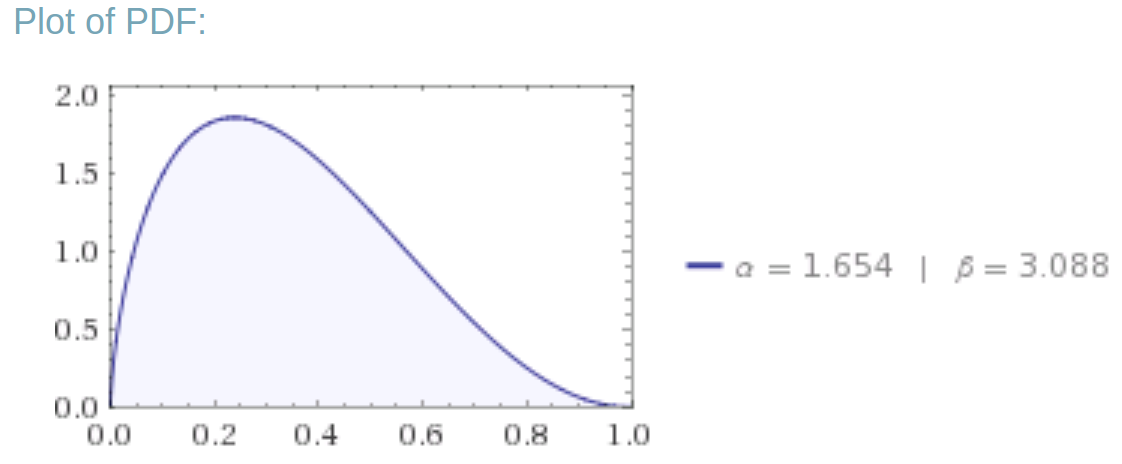
\includegraphics[scale=0.3]{figs/product_appeal_dist.png}
\end{center}

%TCIMACRO{\TeXButton{EndFrame}{\end{frame}}}%
%BeginExpansion
\end{frame}%
%EndExpansion
%TCIMACRO{\TeXButton{BeginFrame}{\begin{frame}}}%
%BeginExpansion
\begin{frame}%
%EndExpansion

\QTR{frametitle}{Parameters}

\begin{center}
{\small 
\begin{tabular}{llrr}
\multicolumn{4}{c}{\textbf{Parameters Estimated using indirect inference (}$%
\Lambda $\textbf{)}} \\ \hline\hline
& \textit{Parameter} & \textit{value} & \textit{std. error} \\ \cline{2-4}
demand shock jump hazard                                     & $\lambda _{y}$       & 0.501    &       \\
demand shock jump size                                       & $\Delta ^{y}$        & 0.037    &       \\
shipment order arrival hazard                                & $\lambda _{b}$       & 1.216    &       \\
std. deviation, log firm type                                & $\sigma _{\varphi }$ & 0.628    &       \\
network effect parameter                                     & $\gamma $            & 0.011    &       \\
\multicolumn{1}{c}{search cost function curvature parameter} & $\kappa _{1}$        & 0.041    &       \\
search cost function scale parameter                         & $\kappa _{0}$        & 132.533  &       \\
\hline
\end{tabular}%
}
\end{center}

\begin{itemize}
\item {\small convexity of search cost function is important}

\item {\small cost of search at hazard }$s=0.6${\small : }${\small \$6,829}$%
{\small \ when }$a=0${\small ; }${\small \$5614}${\small \ when }$a=1${\small ; }${\small \$2,888}${\small \ when } $a=20.$

\item {\small "lock-in" effect}
\end{itemize}

%TCIMACRO{\TeXButton{EndFrame}{\end{frame}}}%
%BeginExpansion
\end{frame}%
%EndExpansion
%TCIMACRO{\TeXButton{BeginFrame}{\begin{frame}}}%
%BeginExpansion
\begin{frame}%
%EndExpansion

\QTR{frametitle}{Parameters}

\QTR{framesubtitle}{restricted models}

%TCIMACRO{%
%\FRAME{ftbpF}{4.0966in}{2.2087in}{0pt}{}{}{Figure}{%
%\special{language "Scientific Word";type "GRAPHIC";maintain-aspect-ratio TRUE;display "USEDEF";valid_file "T";width 4.0966in;height 2.2087in;depth 0pt;original-width 7.2705in;original-height 3.9003in;cropleft "0";croptop "1";cropright "1";cropbottom "0";tempfilename 'MVUDQX07.wmf';tempfile-properties "PR";}}}%
%BeginExpansion
%EndExpansion
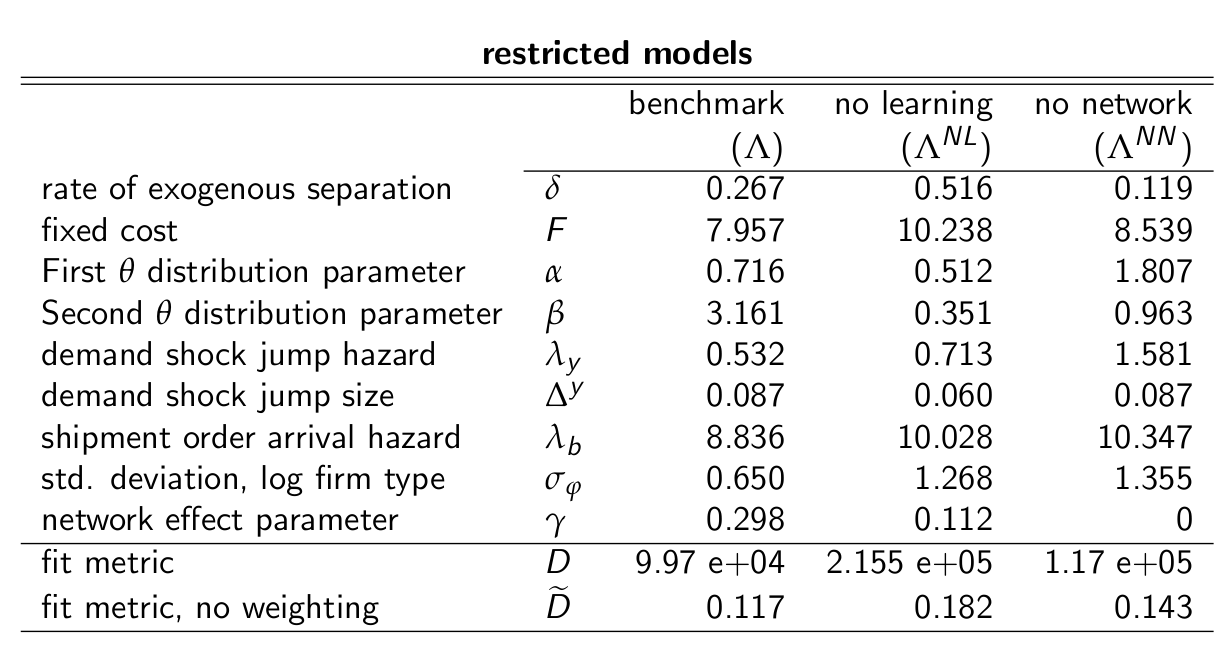
\includegraphics[scale=0.27]{figs/restricted.png}

\begin{itemize}
\item {\small no-learning model, treats firms as knowing their exact }$%
\theta ^{f}${\small \ draws}

\item {\small no-network model shuts down reputation effects by imposing }$%
\gamma =0$
\end{itemize}

%TCIMACRO{\TeXButton{EndFrame}{\end{frame}}}%
%BeginExpansion
\end{frame}%
%EndExpansion
%TCIMACRO{\TeXButton{BeginFrame}{\begin{frame}}}%
%BeginExpansion
\begin{frame}%
%EndExpansion

\QTR{frametitle}{Parameters}

\QTR{framesubtitle}{The no-learning model}

\begin{itemize}
\item Rapid turnover of novice exporters less likely:

\begin{itemize}
\item discourages inexperienced low-$\theta ^{f}$ firms from exploring
foreign markets

\item eliminates learning-based exit.
\end{itemize}

\item High-$\theta ^{f}$ firms do not intensify their search efforts as they
receive positive feedback.

\item Lower productivity firms induced to participate in export markets by a

\begin{itemize}
\item rightward shift in $\theta ^{f}$ distribution and

\item higher values for $\Pi ^{f}$ and $\lambda _{b}$
\end{itemize}

\item Match failure rates and market exit rates are sustained by

\begin{itemize}
\item higher values for $F,$ $\delta ,$ and $\lambda _{y}$.
\end{itemize}

\item Model badly overstates the share of firms that export, overstates the
relationship between sales per client and number of clients.
\end{itemize}

%TCIMACRO{\TeXButton{EndFrame}{\end{frame}}}%
%BeginExpansion
\end{frame}%
%EndExpansion
%TCIMACRO{\TeXButton{BeginFrame}{\begin{frame}}}%
%BeginExpansion
\begin{frame}%
%EndExpansion

\QTR{frametitle}{Parameters}

\QTR{framesubtitle}{The no-network model}

\begin{itemize}
\item Model moves part way toward matching the Pareto shape by reducing the
convexity of the search cost function, $\kappa _{1}.$

\item This is an imperfect fix because all exporters are equally affected by 
$\kappa _{1}$, not just the larger ones.

\item Various other adjustments occur, including:

\begin{itemize}
\item modest increase in $F$,

\item rightward shift in the $\theta $ distribution, an

\item increase in the variance of $\varphi ,$

\item increase in the jump hazard for buyer shocks, $\lambda _{y}$
\end{itemize}

\item Client distribution is far from Pareto: model is unable to explain the
existence of very large exporters; overstates the fraction of firms that
export.
\end{itemize}

%TCIMACRO{\TeXButton{EndFrame}{\end{frame}}}%
%BeginExpansion
\end{frame}%
%EndExpansion
%TCIMACRO{\TeXButton{BeginFrame}{\begin{frame}}}%
%BeginExpansion
\begin{frame}%
%EndExpansion

\QTR{frametitle}{Learning and the policy function}

\begin{itemize}
\item Fix productivity: search intensity as a function of past successes and failures
%TCIMACRO{%
%\FRAME{ftbpF}{3.1237in}{2.4284in}{0pt}{}{}{original_policy_no_suc.eps}{%
%\special{language "Scientific Word";type "GRAPHIC";maintain-aspect-ratio TRUE;display "USEDEF";valid_file "F";width 3.1237in;height 2.4284in;depth 0pt;original-width 7.1676in;original-height 5.5642in;cropleft "0";croptop "1";cropright "1";cropbottom "0";filename '../current docs/Eaton project/figures/eps_plots/original_policy_no_suc.eps';file-properties "NPEU";}}}%
%BeginExpansion
%EndExpansion
\end{itemize}

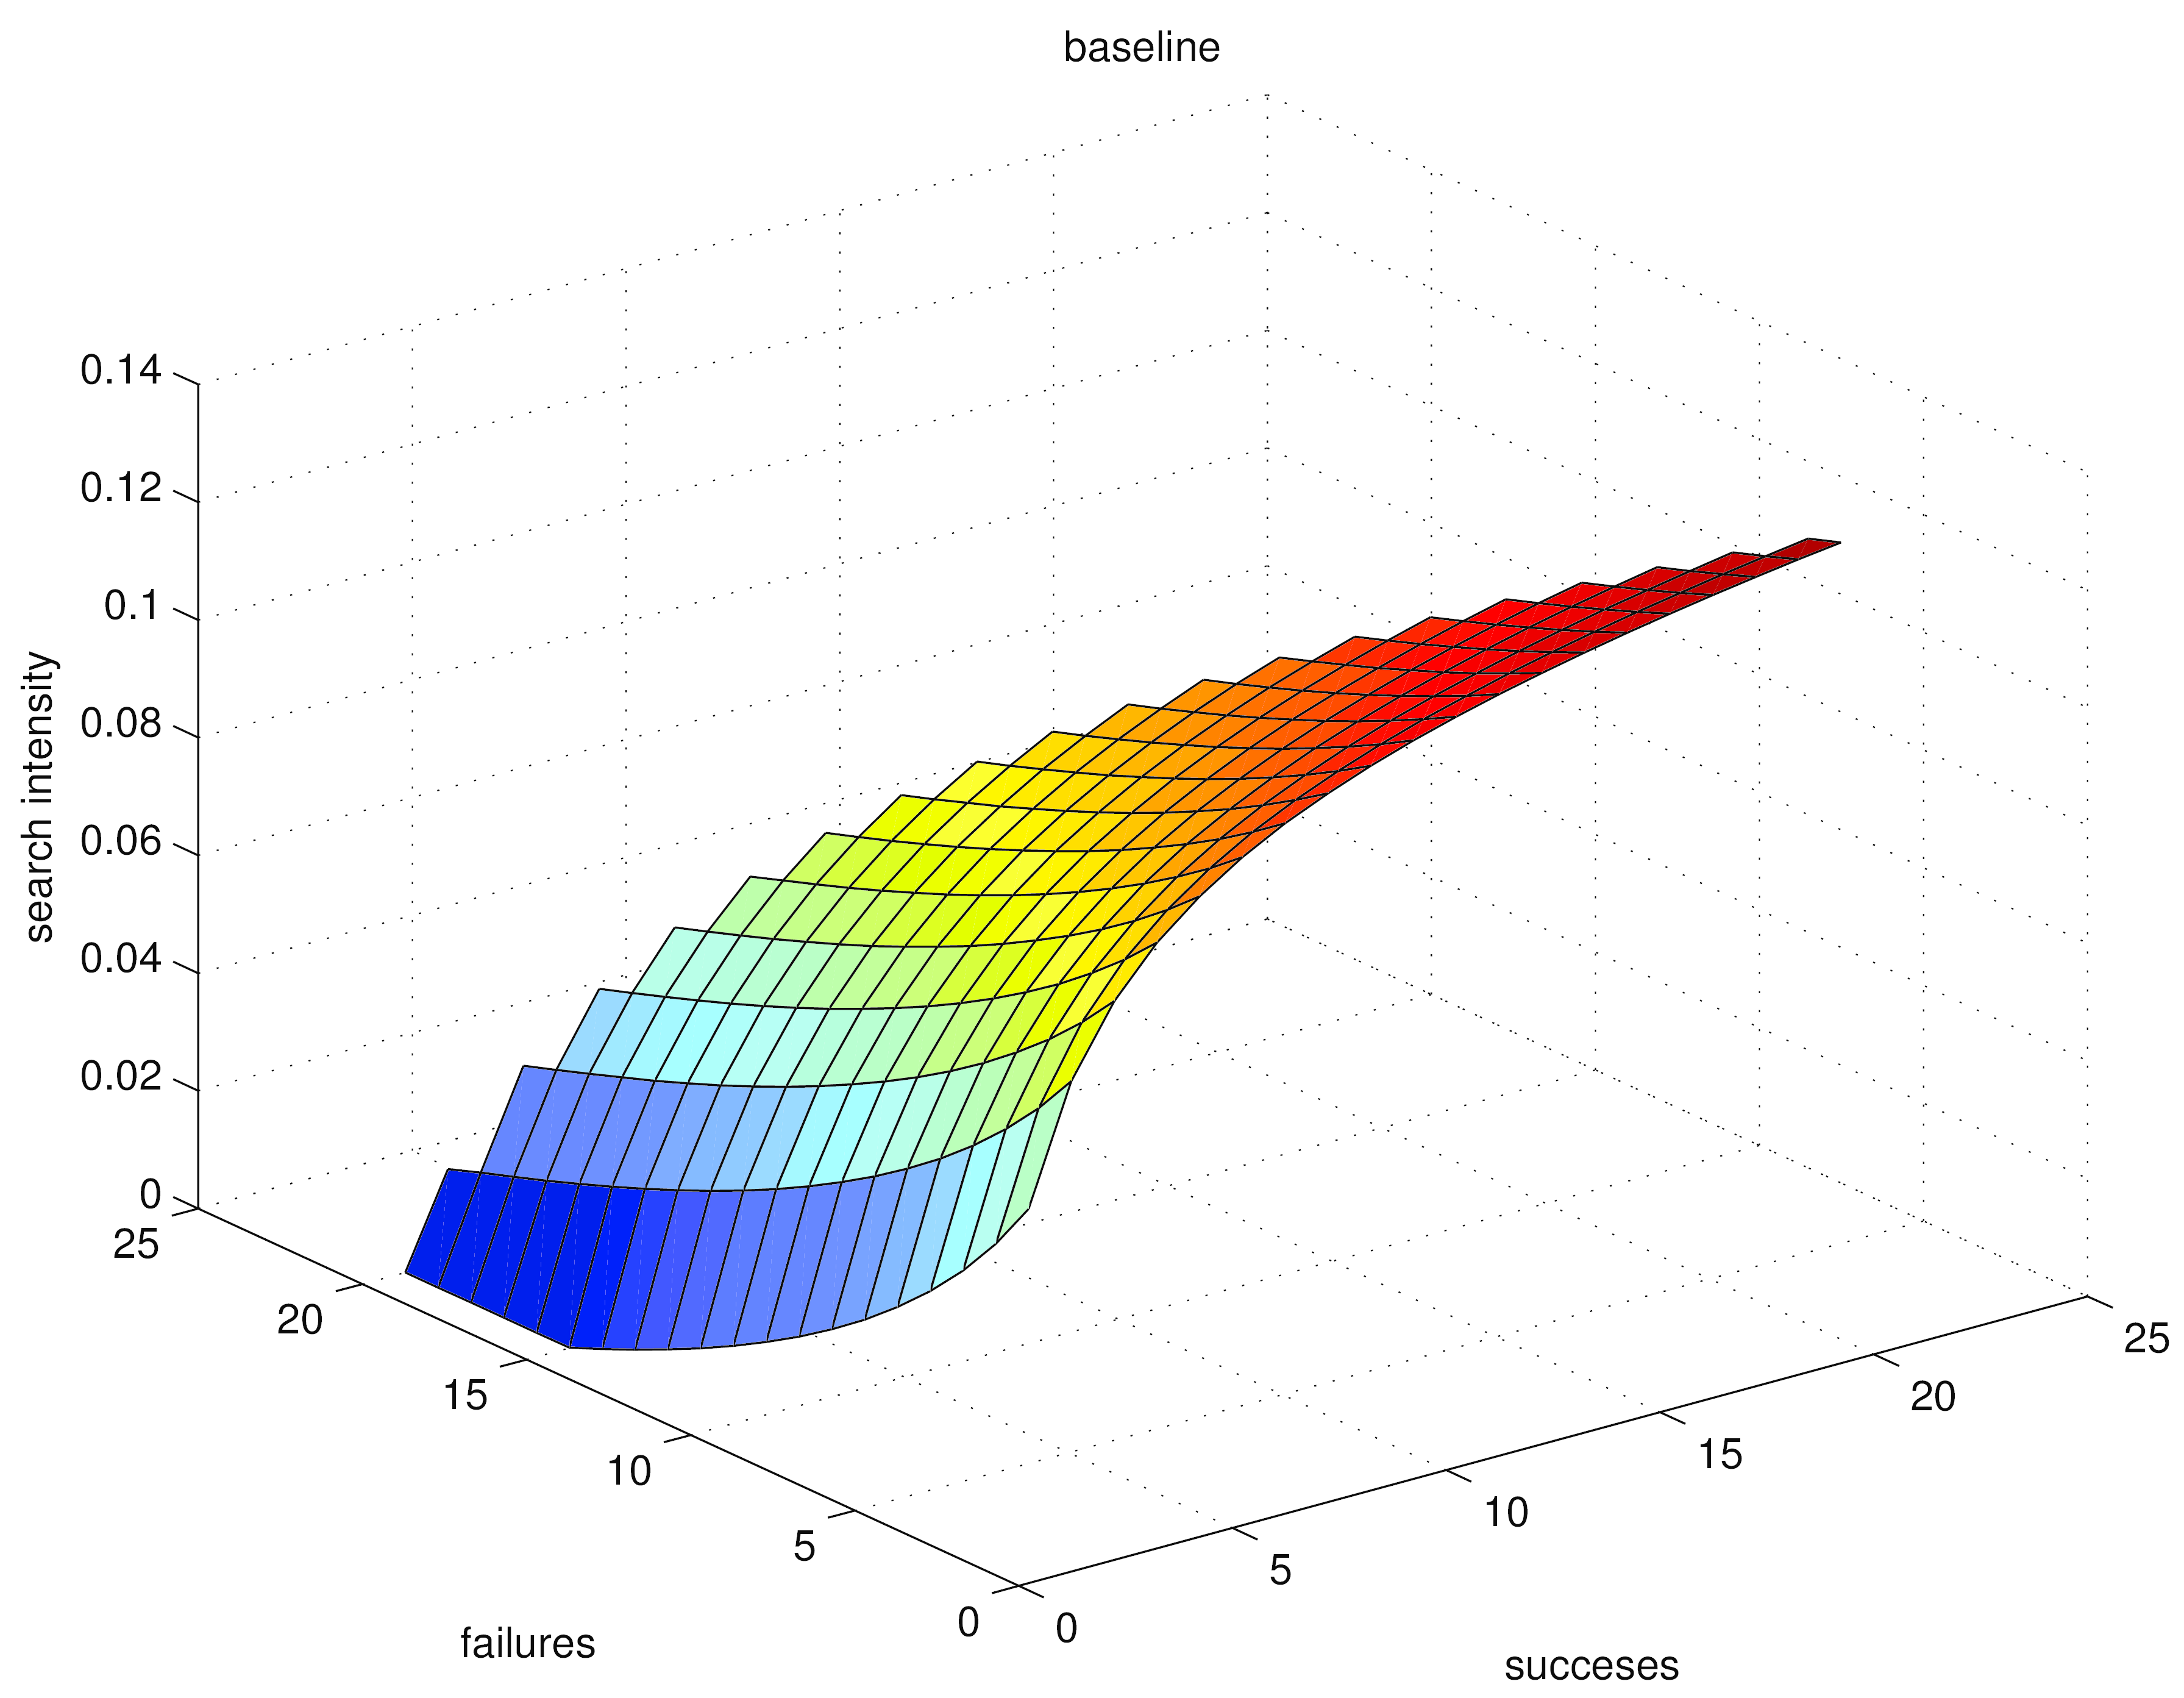
\includegraphics[scale=0.07]{figs/baseline_policy.png}

%TCIMACRO{\TeXButton{EndFrame}{\end{frame}}}%
%BeginExpansion
\end{frame}%
%EndExpansion
%TCIMACRO{\TeXButton{BeginFrame}{\begin{frame}}}%
%BeginExpansion
\begin{frame}%
%EndExpansion

\QTR{frametitle}{Learning and the policy function: 2D}

\begin{itemize}
\item Fix productivity: search intensity as a function of past successes and failures
%TCIMACRO{%
%\FRAME{ftbpF}{3.3399in}{2.6264in}{0pt}{}{}{original_policy.eps}{%
%\special{language "Scientific Word";type "GRAPHIC";maintain-aspect-ratio TRUE;display "USEDEF";valid_file "F";width 3.3399in;height 2.6264in;depth 0pt;original-width 7.0854in;original-height 5.5642in;cropleft "0";croptop "1";cropright "1";cropbottom "0";filename '../current docs/Eaton project/figures/eps_plots/original_policy.eps';file-properties "NPEU";}}}%
%BeginExpansion
%EndExpansion
\end{itemize}

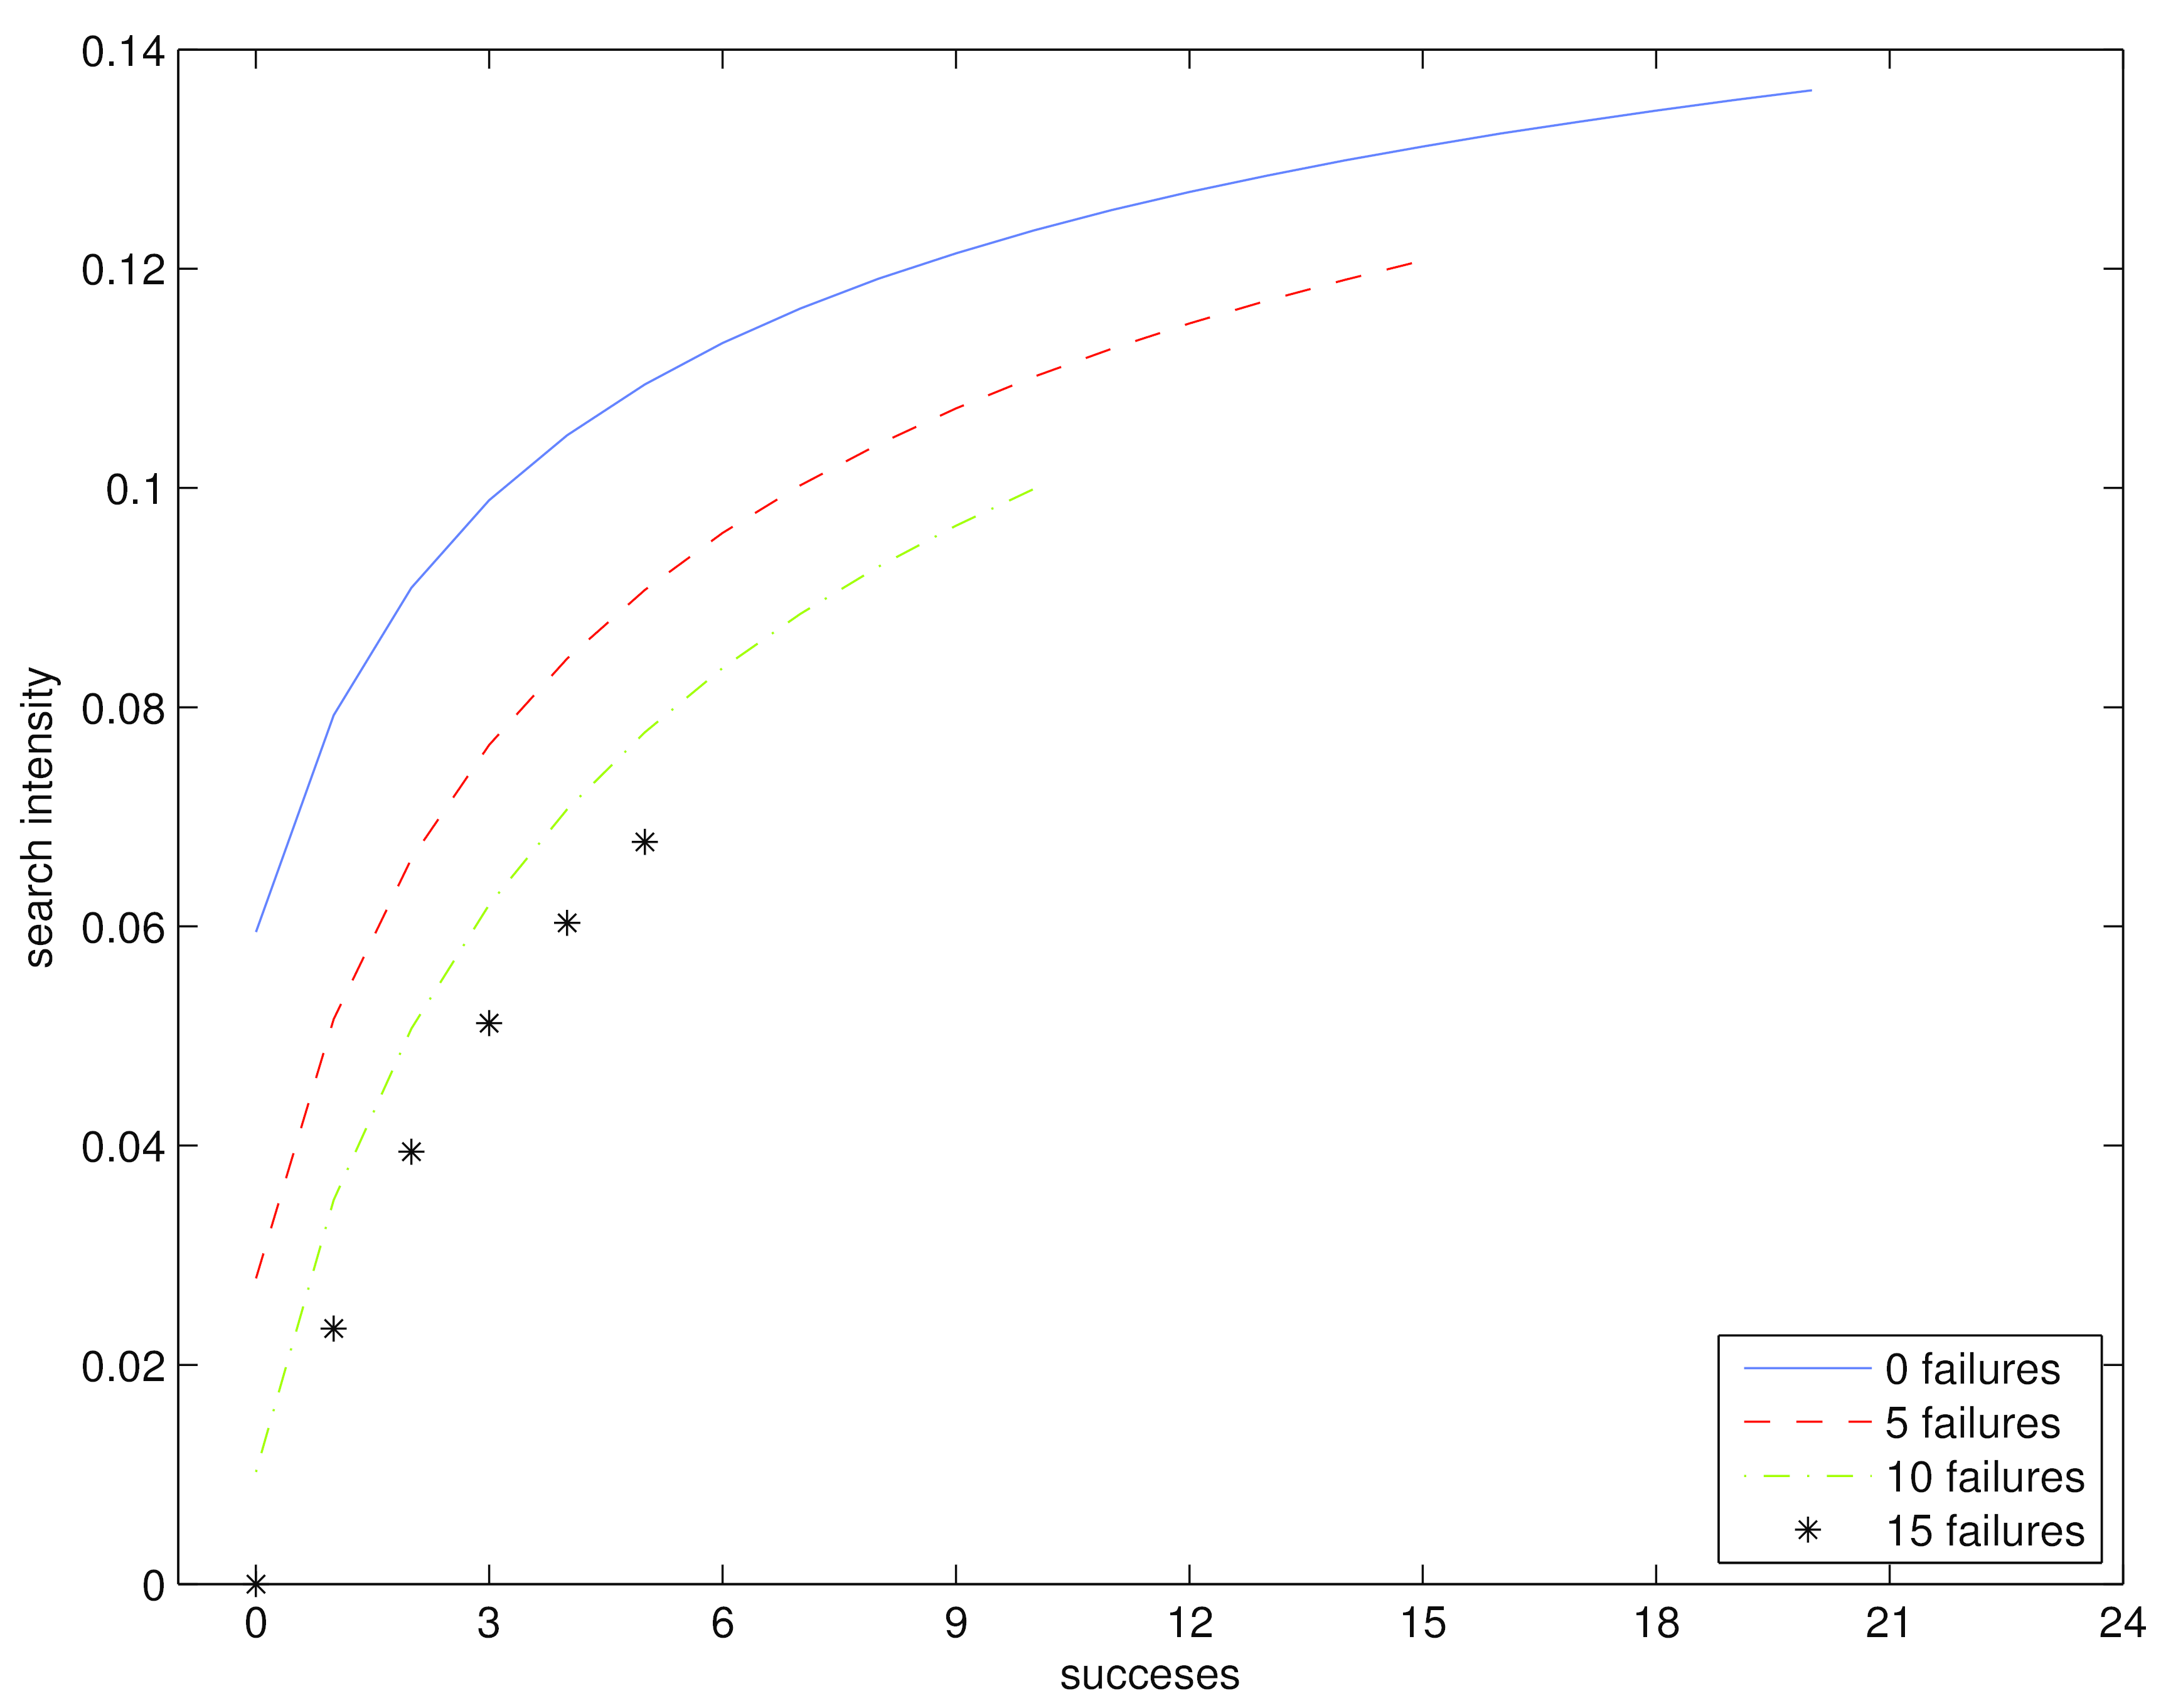
\includegraphics[scale=0.07]{figs/baseline_policy_2d.png}

%TCIMACRO{\TeXButton{EndFrame}{\end{frame}}}%
%BeginExpansion
\end{frame}%
%EndExpansion
%TCIMACRO{\TeXButton{BeginFrame}{\begin{frame}}}%
%BeginExpansion
\begin{frame}%
%EndExpansion

\QTR{frametitle}{Productivity and search}

\begin{itemize}
\item Fix successes at zero: search intensity as a function of productivity and failures
%TCIMACRO{%
%\FRAME{ftbpF}{3.1237in}{2.4284in}{0pt}{}{}{original_policy_no_suc.eps}{%
%\special{language "Scientific Word";type "GRAPHIC";maintain-aspect-ratio TRUE;display "USEDEF";valid_file "F";width 3.1237in;height 2.4284in;depth 0pt;original-width 7.1676in;original-height 5.5642in;cropleft "0";croptop "1";cropright "1";cropbottom "0";filename '../current docs/Eaton project/figures/eps_plots/original_policy_no_suc.eps';file-properties "NPEU";}}}%
%BeginExpansion
%EndExpansion
\end{itemize}

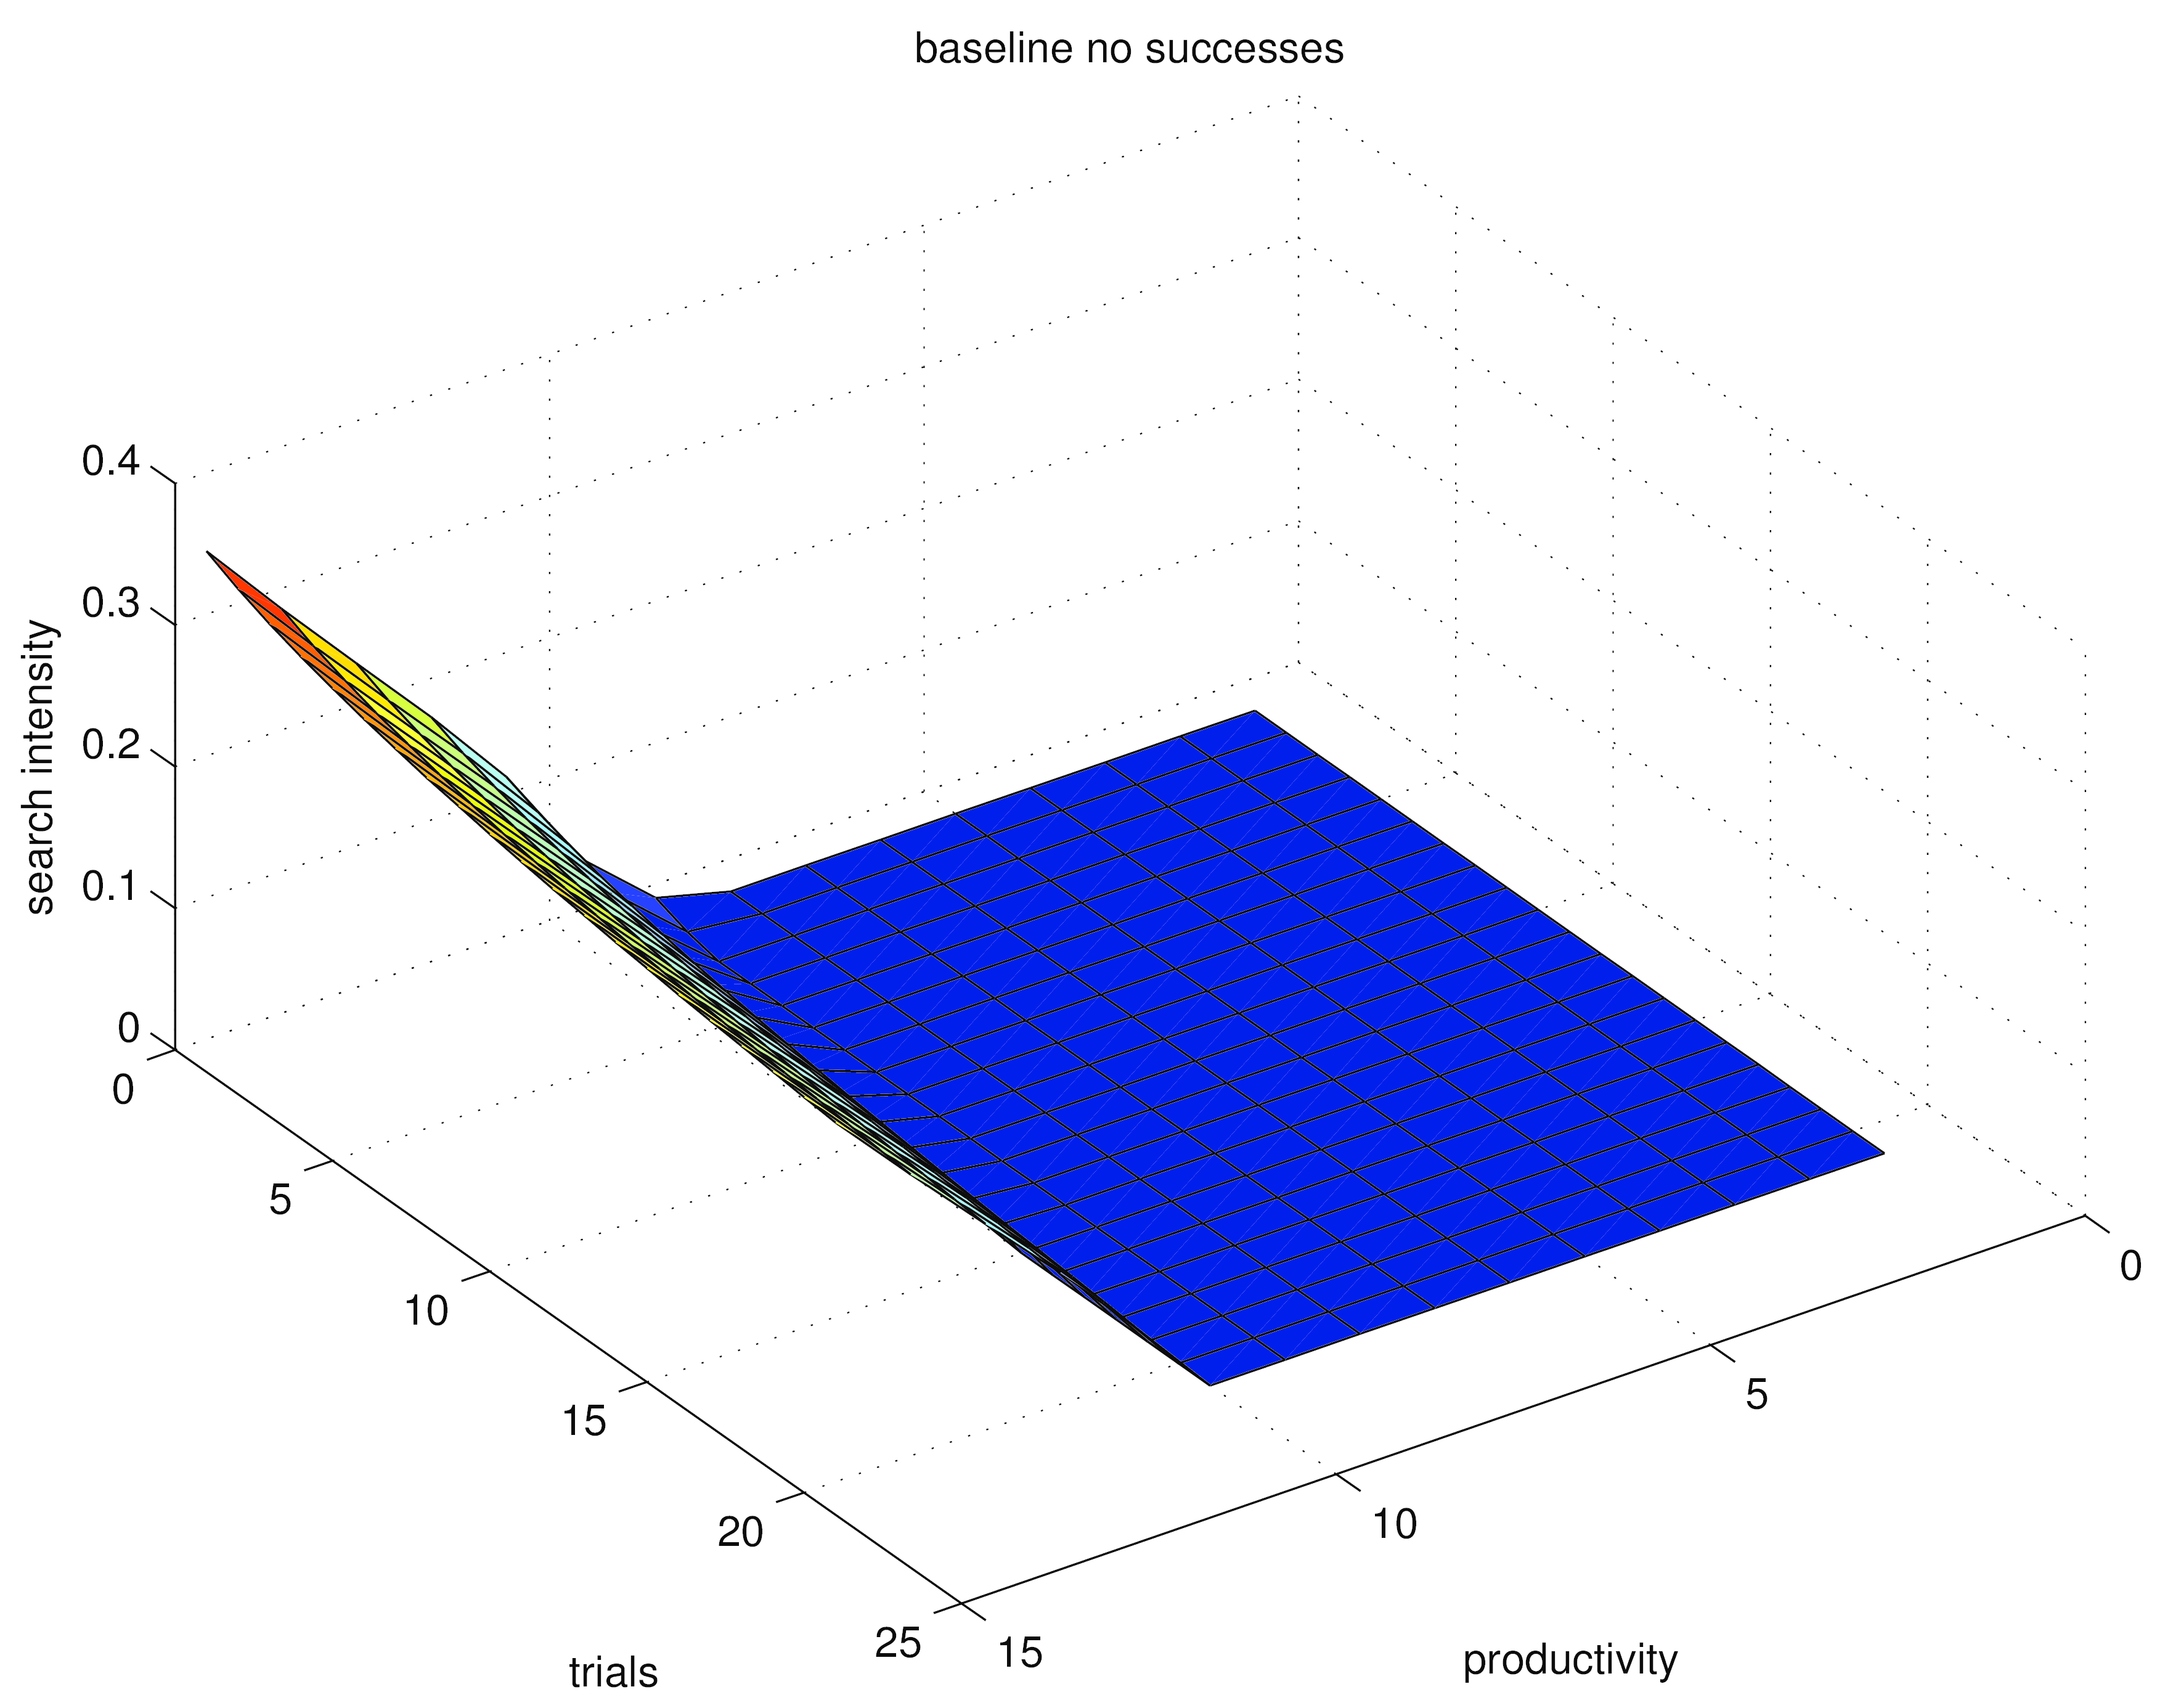
\includegraphics[scale=0.07]{figs/baseline_policy_no_suc.png}

%TCIMACRO{\TeXButton{EndFrame}{\end{frame}}}%
%BeginExpansion
\end{frame}%
%EndExpansion
%TCIMACRO{\TeXButton{BeginFrame}{\begin{frame}}}%
%BeginExpansion
\begin{frame}%
%EndExpansion

\QTR{frametitle}{Learning and the policy function: 2D}

\begin{itemize}
\item Fix successes at zero: search intensity as a function of productivity and failures
%TCIMACRO{%
%\FRAME{ftbpF}{3.3399in}{2.6264in}{0pt}{}{}{original_policy.eps}{%
%\special{language "Scientific Word";type "GRAPHIC";maintain-aspect-ratio TRUE;display "USEDEF";valid_file "F";width 3.3399in;height 2.6264in;depth 0pt;original-width 7.0854in;original-height 5.5642in;cropleft "0";croptop "1";cropright "1";cropbottom "0";filename '../current docs/Eaton project/figures/eps_plots/original_policy.eps';file-properties "NPEU";}}}%
%BeginExpansion
%EndExpansion
\end{itemize}

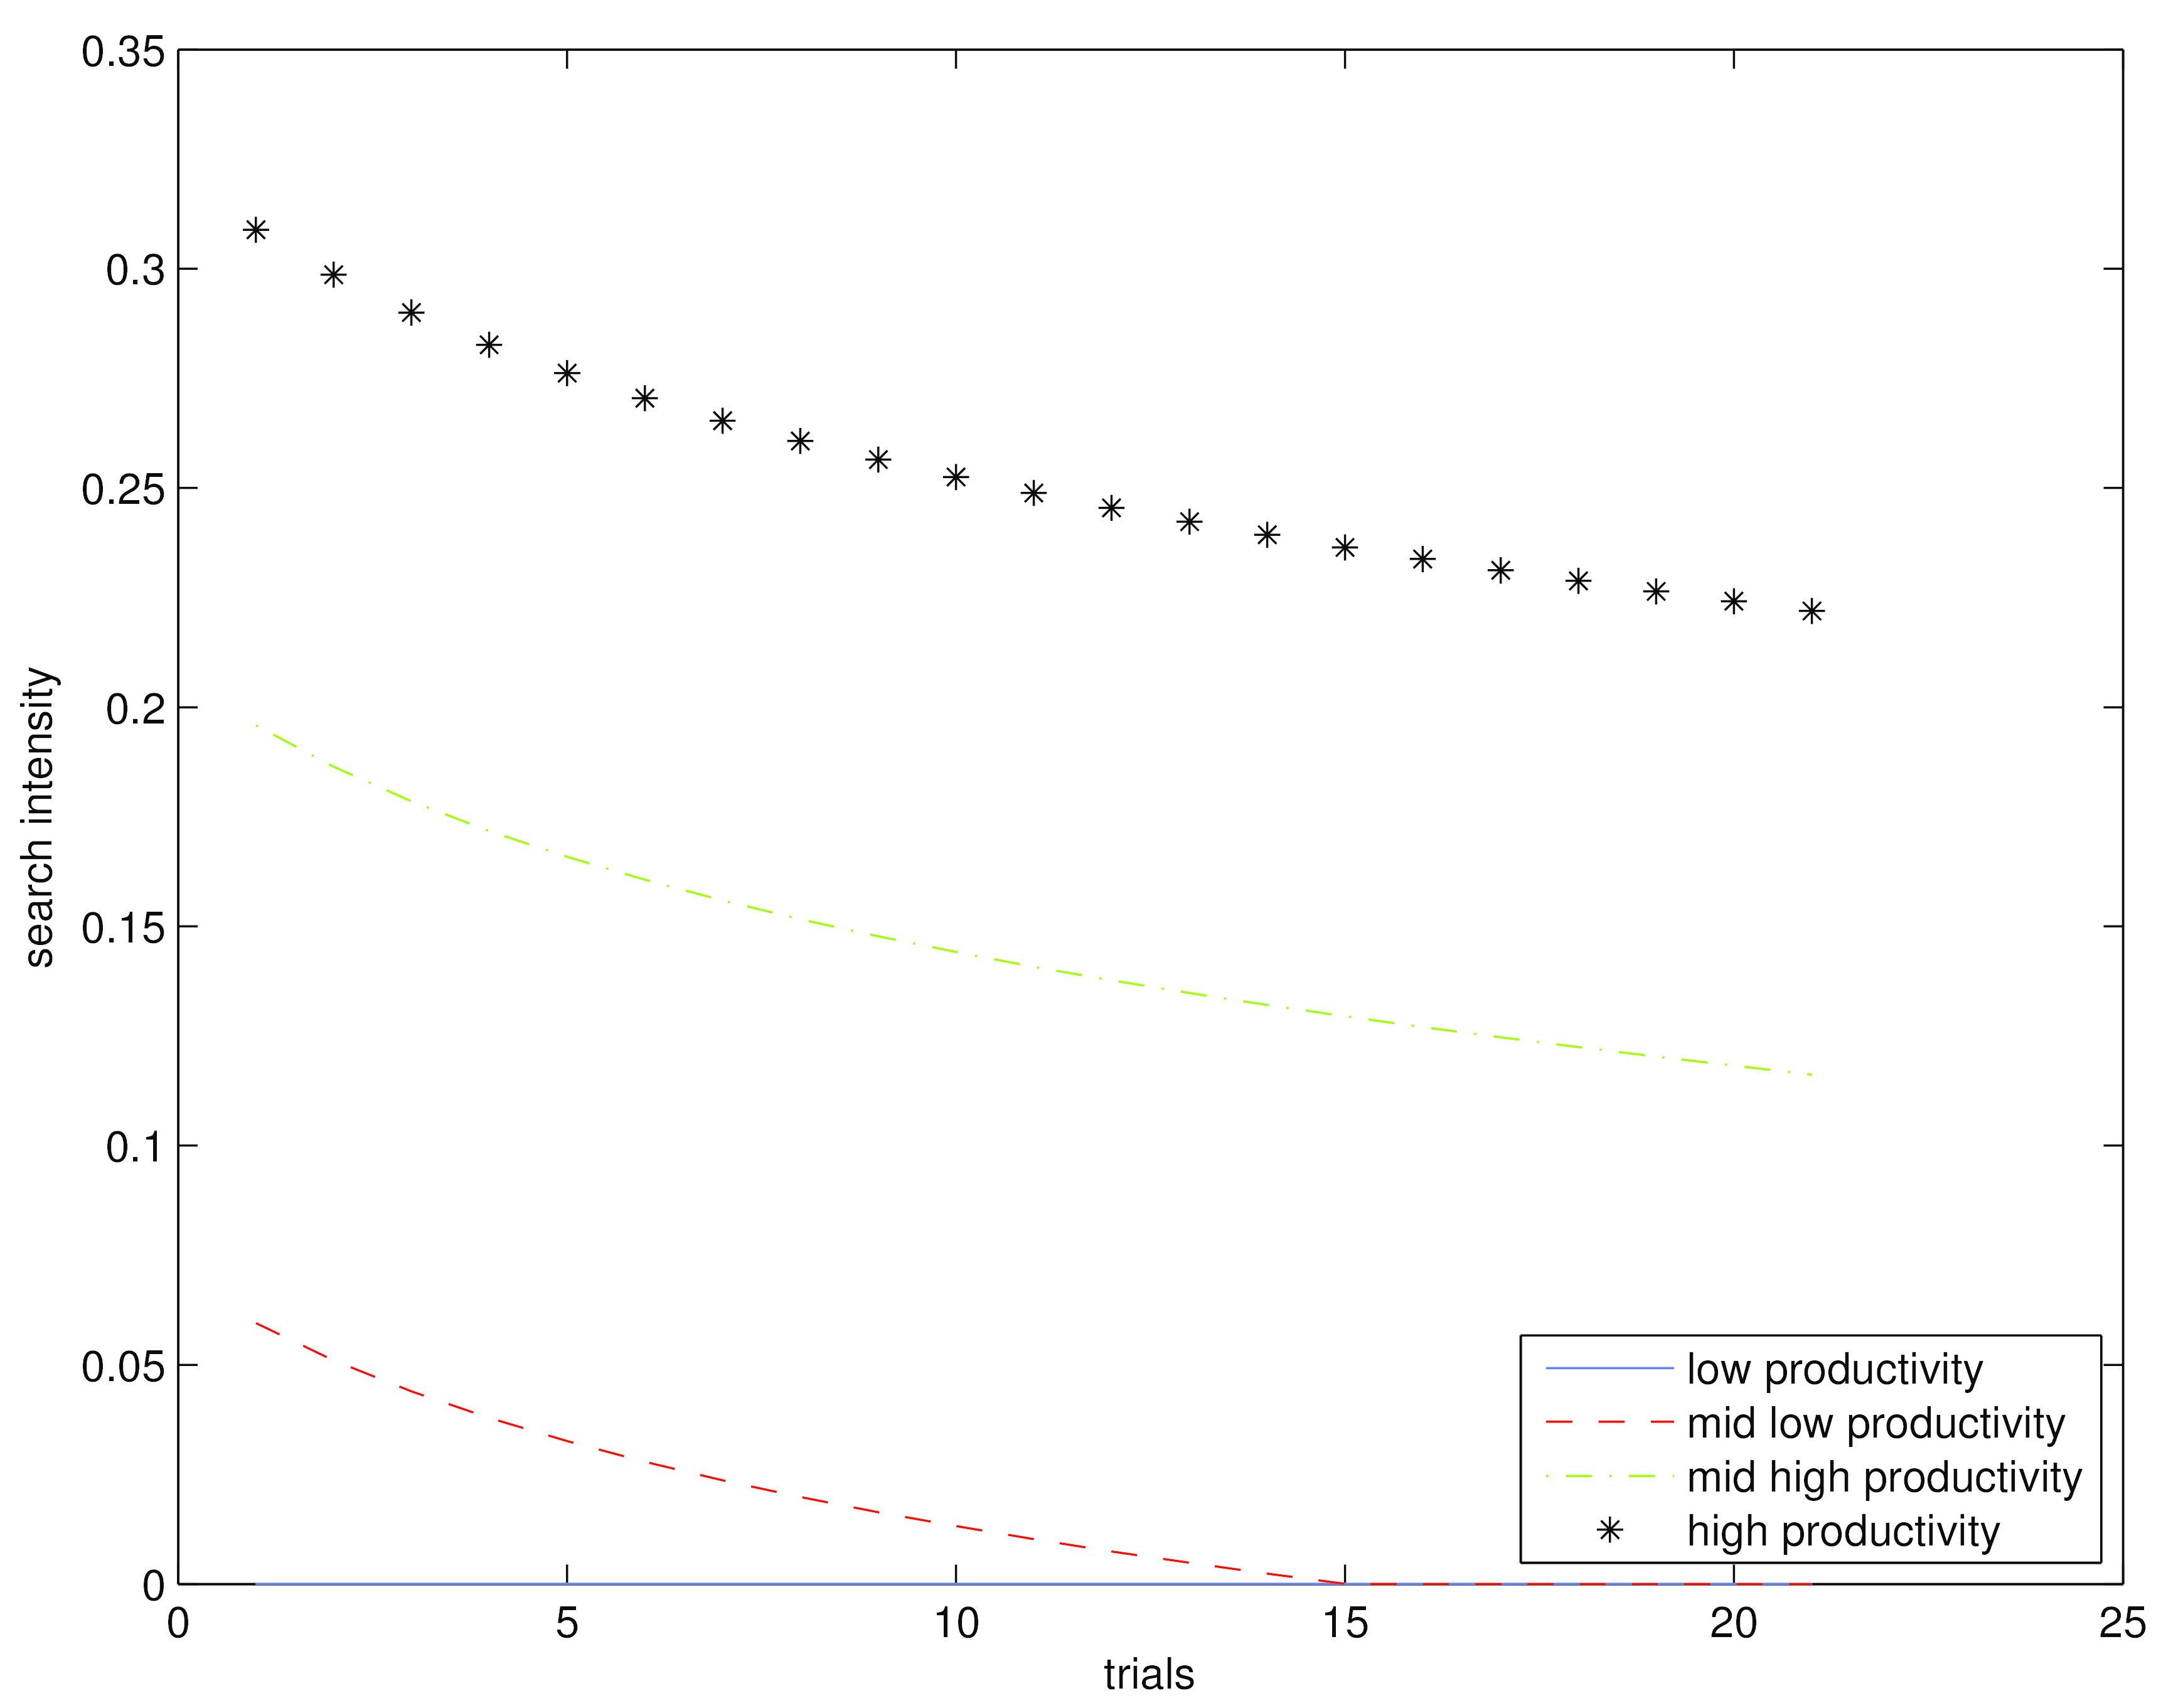
\includegraphics[scale=0.07]{figs/baseline_policy_no_suc_2d.png}

%TCIMACRO{\TeXButton{EndFrame}{\end{frame}}}%
%BeginExpansion
\end{frame}%
\begin{frame}%
%EndExpansion

\QTR{frametitle}{A 20\% increase in foreign market size}

\begin{center}
%TCIMACRO{%
%\FRAME{ftbpF}{3.7939in}{2.8487in}{0pt}{}{}{mac_bump_subplot.eps}{%
%\special{language "Scientific Word";type "GRAPHIC";maintain-aspect-ratio TRUE;display "USEDEF";valid_file "F";width 3.7939in;height 2.8487in;depth 0pt;original-width 6.96in;original-height 5.2157in;cropleft "0";croptop "1";cropright "1";cropbottom "0";filename '../current docs/Eaton project/plots 6-1-13/mac_bump_subplot.eps';file-properties "NPEU";}}}%
%BeginExpansion
%EndExpansion
    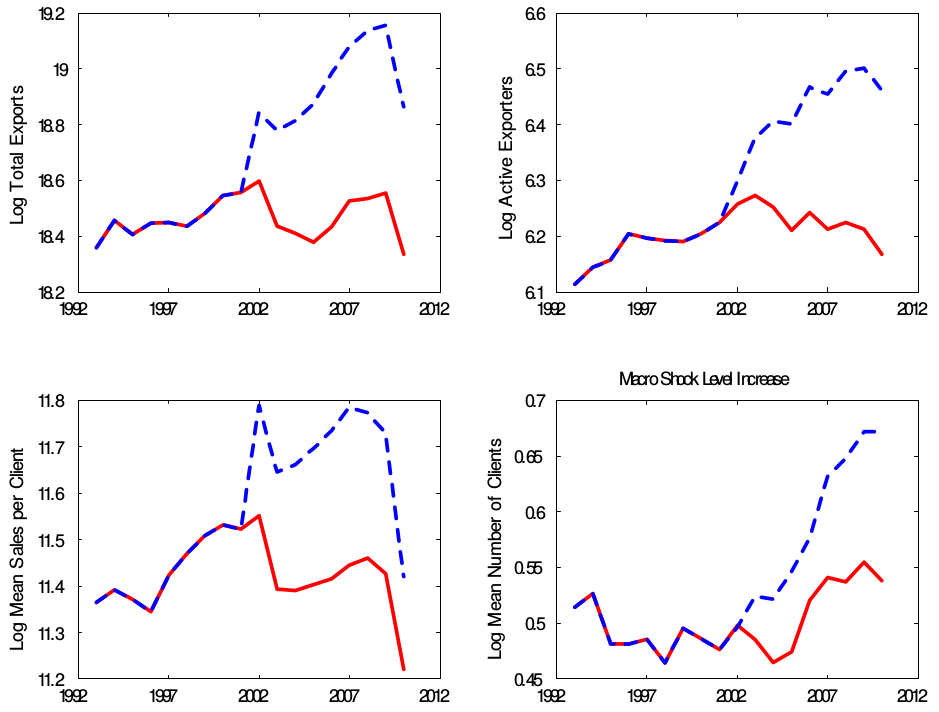
\includegraphics[scale=0.3]{figs/increase_in_foreign_market_size.png}
\end{center}

%TCIMACRO{\TeXButton{EndFrame}{\end{frame}}}%
%BeginExpansion
\end{frame}%
%EndExpansion
%TCIMACRO{\TeXButton{BeginFrame}{\begin{frame}}}%
%BeginExpansion
\begin{frame}%
%EndExpansion

\begin{center}
\QTR{frametitle}{A 20\% reduction in search costs}%
%TCIMACRO{%
%\FRAME{ftbpF}{3.6902in}{2.7709in}{0pt}{}{}{search_dec_subplot.eps}{%
%\special{language "Scientific Word";type "GRAPHIC";maintain-aspect-ratio TRUE;display "USEDEF";valid_file "F";width 3.6902in;height 2.7709in;depth 0pt;original-width 6.96in;original-height 5.2157in;cropleft "0";croptop "1";cropright "1";cropbottom "0";filename '../current docs/Eaton project/plots 6-1-13/search_dec_subplot.eps';file-properties "NPEU";}}}%
%BeginExpansion
%EndExpansion
    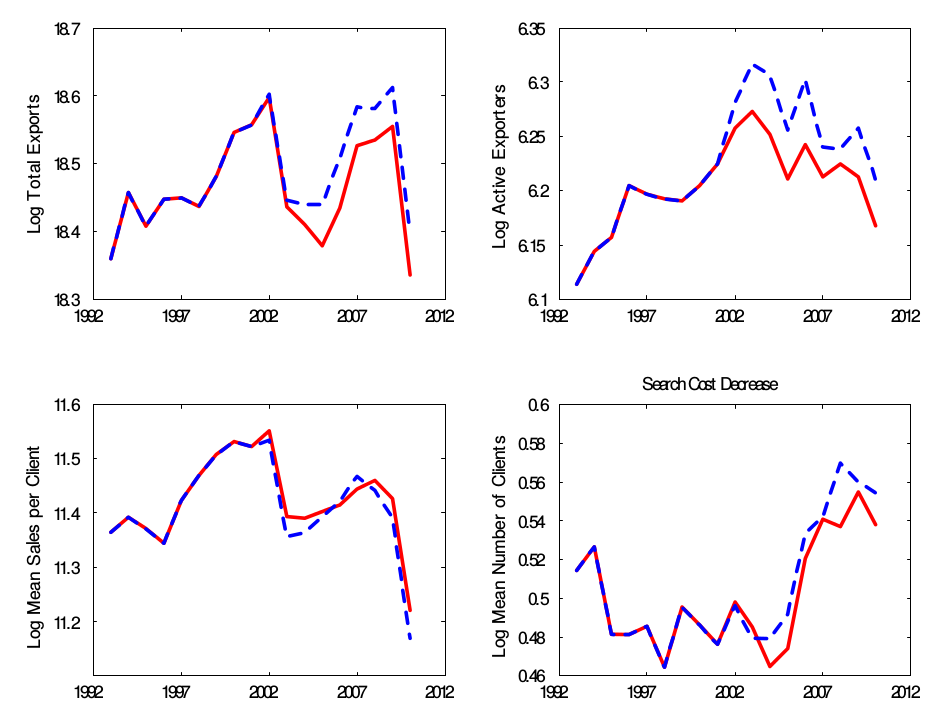
\includegraphics[scale=0.3]{figs/reduction_in_search_costs.png}
\end{center}

%TCIMACRO{\TeXButton{EndFrame}{\end{frame}}}%
%BeginExpansion
\end{frame}%
%EndExpansion
%TCIMACRO{\TeXButton{BeginFrame}{\begin{frame}}}%
%BeginExpansion
\begin{frame}%
%EndExpansion

\QTR{frametitle}{A 20\% reduction in fixed costs}

\begin{center}
%TCIMACRO{%
%\FRAME{ftbpF}{3.7386in}{2.8072in}{0pt}{}{}{cost_dec_subplot.eps}{%
%\special{language "Scientific Word";type "GRAPHIC";maintain-aspect-ratio TRUE;display "USEDEF";valid_file "F";width 3.7386in;height 2.8072in;depth 0pt;original-width 6.96in;original-height 5.2157in;cropleft "0";croptop "1";cropright "1";cropbottom "0";filename '../current docs/Eaton project/plots 6-1-13/cost_dec_subplot.eps';file-properties "NPEU";}}}%
%BeginExpansion
%EndExpansion
    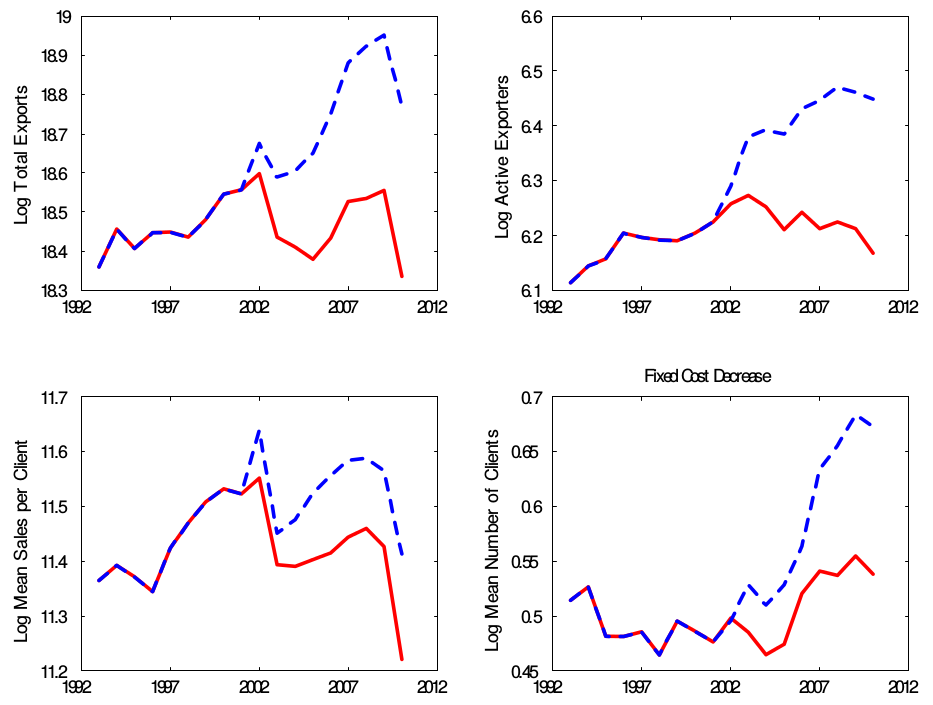
\includegraphics[scale=0.3]{figs/reduction_in_fixed_costs.png}
\end{center}

%TCIMACRO{\TeXButton{EndFrame}{\end{frame}}}%
%BeginExpansion
\end{frame}%
%EndExpansion
%TCIMACRO{\TeXButton{BeginFrame}{\begin{frame}}}%
%BeginExpansion
%EndExpansion
%TCIMACRO{\TeXButton{BeginFrame}{\begin{frame}}}%
%BeginExpansion
\begin{frame}%
%EndExpansion

\QTR{frametitle}{Summary}

\begin{itemize}
\item Micro patterns of transactions and buyer-seller relationships through
the lens of the model:

\begin{itemize}
\item Large volume of small scale exporters explained by large volume of
inexperienced firms, searching at a low level.

\item High exit rate reflects short lifespan of typical match, combined with
low-level search and learning about product appeal.

\item Small number of major exporters reflects combination of skewed
distribution of product appeal and reputation effects.
\end{itemize}

\item Search costs, multi-period matches, learning, and reputation effects
combine to provide an explanation for hysteresis in trade.

\begin{itemize}
\item Reputation effects appear to be particularly important.

\item Since learning is mainly relevant for new, marginal players, probably
doesn't have a big effect on short-run export dynamics.
\end{itemize}
\end{itemize}

%TCIMACRO{\TeXButton{EndFrame}{\end{frame}}}%
%BeginExpansion
\end{frame}%
%EndExpansion
%TCIMACRO{\TeXButton{BeginFrame}{\begin{frame}}}%
%BeginExpansion
\begin{frame}%
%EndExpansion

\QTR{frametitle}{A Digression: hazards}

\begin{itemize}
\item From the perspective of time 0, let the probability that an event will
occur before time $t$ be described by the exponential distribution:%
\[
F[t]=1-e^{-qt} 
\]

\item The likelihood of the event happening exactly at $t$ (the "hazard
rate" at $t$) is then: 
\[
\frac{f(t)}{1-F(t)}=\frac{qe^{-qt}}{e^{-qt}}=q 
\]

\item This hazard rate doesn't depend upon $t.$
\end{itemize}

\label{appendix}

%TCIMACRO{\TeXButton{EndFrame}{\end{frame}}}%
%BeginExpansion
\end{frame}%
%EndExpansion
%TCIMACRO{\TeXButton{BeginFrame}{\begin{frame}}}%
%BeginExpansion
\begin{frame}%
%EndExpansion

\QTR{frametitle}{Hazards}

\begin{itemize}
\item Suppose $k$ independent events occur with hazard $q_{1},q_{2},...q_{k}$%
. The probability that none occur before $t$ is: 
\[
\dprod\limits_{j=1}^{k}\left( 1-F_{j}(t)\right) =e^{-t\Sigma _{j}q_{j}} 
\]

\item So by time $t$, at least one event occurs with probability $%
1-e^{-t\Sigma _{j}q_{j}},$ and the likelihood that this happens exactly at $%
t $ is%
\[
\frac{\Sigma _{j}q_{j}\left[ e^{-t\Sigma _{j}q_{j}}\right] }{e^{-t\Sigma
_{j}q_{j}}}=\Sigma _{j}q_{j} 
\]
\end{itemize}

%TCIMACRO{\TeXButton{EndFrame}{\end{frame}}}%
%BeginExpansion
\end{frame}%
%EndExpansion
%TCIMACRO{\TeXButton{BeginFrame}{\begin{frame}}}%
%BeginExpansion
\begin{frame}%
%EndExpansion

\label{pihat_derivation}

\QTR{frametitle}{Relationship dynamics}

\QTR{framesubtitle}{Markov jump processes}

\begin{itemize}
\item $x$ (market-wide) follows Markov jump process, hazard $q_{xx^{\prime
}}^{X}$ of transiting from state $x$ to state $x^{\prime }.$

\item $y$ (match-specific) follows Markov jump process, hazard $%
q_{yy^{\prime }}^{Y}$ of transiting from state $y$ to state $y^{\prime }$.

\item $\lambda _{x}^{X}=\sum_{x^{\prime }\neq x}q_{xx^{\prime }}^{X}$ is
hazard of a change in market-wide state $x$

\item $\lambda _{y}^{Y}=\sum_{y^{\prime }\neq y}q_{yy^{\prime }}^{Y}$ is
hazard of a change in match-specific state $y$.

\item $\lambda ^{b}$ is hazard of a new purchase order from existing client.

\item $\tau _{b}$ time until the next change in state, which occurs with
hazard $\lambda ^{b}+\lambda _{x}^{X}+\lambda _{y}^{Y}$
\end{itemize}

%TCIMACRO{\TeXButton{EndFrame}{\end{frame}}}%
%BeginExpansion
\end{frame}%
%EndExpansion
%TCIMACRO{\TeXButton{BeginFrame}{\begin{frame}}}%
%BeginExpansion
\begin{frame}%
%EndExpansion

\QTR{frametitle}{Relationship dynamics}

\QTR{framesubtitle}{the continuation value}

\begin{itemize}
\item $\delta $ exogenous hazard of relationship death.

\item $\rho $ seller's discount rate.
\end{itemize}

Continuation value of a business relationship in state $(x,y)$ for a type-$%
\varphi $ exporter :%
\begin{eqnarray*}
\widehat{\pi }_{\varphi }(x,y) &=&\mathbf{E}_{\tau _{b}}\left[ e^{-(\rho
+\delta )\tau _{b}}\frac{1}{\lambda ^{b}+\lambda _{x}^{X}+\lambda _{y}^{Y}}%
\right. \\
&&\left. \cdot \left( \sum_{x^{\prime }\neq x}q_{xx^{\prime }}^{X}\widehat{%
\pi }_{\varphi }(x^{\prime },y)+\sum_{y^{\prime }\neq y}q_{yy^{\prime }}^{Y}%
\widehat{\pi }_{\varphi }(x,y^{\prime })+\lambda ^{b}\widetilde{\pi }%
_{\varphi }(x,y)\right) \right] \\
&=&\frac{1}{h}\left( \sum_{x^{\prime }\neq x}q_{xx^{\prime }}^{X}\widehat{%
\pi }_{\varphi }(x^{\prime },y)+\sum_{y^{\prime }\neq y}q_{yy^{\prime }}^{Y}%
\widehat{\pi }_{\varphi }(x,y^{\prime })+\lambda ^{b}\widetilde{\pi }%
_{\varphi }(x,y)\right)
\end{eqnarray*}%
where%
\[
h=\rho +\delta +\lambda ^{b}+\lambda _{x}^{X}+\lambda _{y}^{Y} 
\]

%TCIMACRO{\TeXButton{EndFrame}{\end{frame}}}%
%BeginExpansion
\end{frame}%
%EndExpansion
%TCIMACRO{\TeXButton{BeginFrame}{\begin{frame}}}%
%BeginExpansion
\begin{frame}%
%EndExpansion

\label{Bayesian_details}

\QTR{frametitle}{Learning about product appeal}

\QTR{framesubtitle}{experience and expected success rates}

\begin{itemize}
\item Suppress market superscripts to reduce clutter.

\item The \textbf{prior distribution} is:%
\[
r(\theta |\alpha ,\beta )=\frac{\Gamma (\alpha +\beta )}{\Gamma (\alpha
)\Gamma (\beta )}\left( \theta \right) ^{\alpha -1}(1-\theta )^{\beta -1}, 
\]

\item \textbf{The likelihood:} Given $\theta ,$ and given that a seller has
met $n$ potential buyers, the probability that $a$ of these buyers were
willing to buy her product is binomially distributed: 
\[
q\left[ a|n,\theta \right] =\binom{n}{a}\left[ \theta \right] ^{a}\left[
1-\theta ^{m}\right] ^{n-a}. 
\]
\end{itemize}

%TCIMACRO{\TeXButton{EndFrame}{\end{frame}}}%
%BeginExpansion
\end{frame}%
%EndExpansion
%TCIMACRO{\TeXButton{BeginFrame}{\begin{frame}}}%
%BeginExpansion
\begin{frame}%
%EndExpansion

\QTR{frametitle}{Learning about product appeal}

\QTR{framesubtitle}{experience and expected success rates}

\begin{itemize}
\item \textbf{The posterior} distribution for $\theta $:%
\[
p(\theta |a,n)\propto q\left[ a|n,\theta \right] \cdot r(\theta |\alpha
,\beta ) 
\]

\item The expected success rate after $a$ successes in $n$ trials is thus: 
\[
\overline{\theta }(a,n)=E\left[ \theta |a,n\right] =\frac{a+\alpha }{%
n+\alpha +\beta } 
\]

\item Sellers base their search intensity on this posterior mean$.$
\end{itemize}

%TCIMACRO{\TeXButton{EndFrame}{\end{frame}}}%
%BeginExpansion
\end{frame}%
%EndExpansion
%TCIMACRO{\TeXButton{BeginFrame}{\begin{frame}}}%
%BeginExpansion
\begin{frame}%
%EndExpansion

\label{optimal_search}

\QTR{frametitle}{Searching for buyers}

\QTR{framesubtitle}{the value of search}

The value of continued search for a type-$\varphi $ firm with $a$ successes
in $n$ meetings is:

\begin{eqnarray*}
&&V_{\varphi }(a,n,x)= \\
&&\max_{s}\mathbf{E}_{\tau _{s}}\left[ -c(s,a)\int_{0}^{\tau _{s}}e^{-\rho
t}dt+\frac{e^{-\rho \tau _{s}}}{s+\lambda _{x}^{X}}\cdot \left(
\sum_{x^{\prime }\neq x}q_{xx^{\prime }}^{X}V_{\varphi ,}(a,n,x^{\prime
})\right. \right. \\
&&\left. \left. 
\begin{array}{c}
\; \\ 
\;%
\end{array}%
+s\left[ \overline{\theta }_{a,n}(\widetilde{\pi }_{\varphi }(x)+V_{\varphi
}(a+1,n+1,x)+(1-\overline{\theta }_{a,n})V_{\varphi }(a,n+1,x)\right]
\right) \right]
\end{eqnarray*}

where:

\begin{itemize}
\item $\lambda _{x}^{X}=\sum_{x^{\prime }\neq x}q_{xx^{\prime }}^{X}$ is the
hazard of any change in the market-wide state $x.$

\item $\tau _{s}$ is the random time until the next search event, which
occurs with hazard $s+\lambda _{x}^{X}$.
\end{itemize}

%TCIMACRO{\TeXButton{EndFrame}{\end{frame}}}%
%BeginExpansion
\end{frame}%
%EndExpansion
%TCIMACRO{\TeXButton{BeginFrame}{\begin{frame}}}%
%BeginExpansion
\begin{frame}%
%EndExpansion

\QTR{frametitle}{Searching for buyers}

\QTR{framesubtitle}{the value of search}

Taking expectations over $\tau _{s}$ yields:%
\begin{eqnarray*}
&&V_{\varphi }(a,n,x) \\
&=&\max_{s}\frac{1}{\rho +s+\lambda _{x}^{X}}\left[ -c(s,a)+\sum_{x^{\prime
}\neq x}q_{xx^{\prime }}^{X}V_{\varphi ,}(a,n,x^{\prime })\right. \\
&&\left. 
\begin{array}{c}
\; \\ 
\;%
\end{array}%
+s\left\{ \overline{\theta }_{a,n}\left[ \widetilde{\pi }_{\varphi
}(x)+V_{\varphi }(a+1,n+1,x)\right] +(1-\overline{\theta }_{a,n})V_{\varphi
}(a,n+1,x)\right\} \right]
\end{eqnarray*}

The first-order condition is thus:%
\begin{eqnarray*}
c_{s}(s^{\ast },a) &=&\overline{\theta }_{a,n}(\widetilde{\pi }_{\varphi
}(x)+V_{\varphi }(a+1,n+1,x)) \\
&&+(1-\overline{\theta }_{a,n})V_{\varphi }(a,n+1,x)-V_{\varphi }(a,n,x).
\end{eqnarray*}

%TCIMACRO{\TeXButton{EndFrame}{\end{frame}}}%
%BeginExpansion
\end{frame}%
%EndExpansion
%TCIMACRO{\TeXButton{BeginFrame}{\begin{frame}}}%
%BeginExpansion
\begin{frame}%
%EndExpansion

\QTR{frametitle}{Searching for buyers}

\QTR{framesubtitle}{when the truth is known: the domestic market}

\begin{itemize}
\item In the domestic market the reward to search depends on $a$ and $n$
only through network effects.

\item The value of search at home is thus simply:%
\[
V_{\varphi }(x)=\max_{s}\frac{1}{\rho +s+\lambda _{x}^{X}}\left[
-c(s,a)+\sum_{x^{\prime }\neq x}q_{xx^{\prime }}^{X}V_{\varphi }(x^{\prime
})+s\theta _{j}\widetilde{\pi }_{\varphi }(x)\right] 
\]

\item The associated first-order condition is:%
\[
c_{s}(s^{\ast },a)=\theta _{j}\widetilde{\pi }_{\varphi }(x). 
\]
\end{itemize}

%TCIMACRO{\TeXButton{EndFrame}{\end{frame}}}%
%BeginExpansion
\end{frame}%
%EndExpansion

\end{document}
